%File: main.tex -- Phantom Claims, AAAI-27 Workshop on Medical World Models (full paper, 6-8 pages + references + appendix)
% Preamble copied from the AAAI-27 author kit (AuthorKit27/AnonymousSubmission2027.tex, https://aaai.org/authorkit27/).
% Every number in the text is a macro from numbers.tex, generated from results/results.jsonl by
% scripts/make_paper_numbers.py (provenance per macro: numbers_provenance.json). Figures: scripts/paper_figures.py.
% For camera-ready, scripts/flatten_paper.py writes the single-file source the kit requires (no \input).
\documentclass[letterpaper]{article} % DO NOT CHANGE THIS
\usepackage[submission]{aaai2027}  % DO NOT CHANGE THIS
\usepackage[hyphens]{url}  % DO NOT CHANGE THIS
\usepackage{graphicx} % DO NOT CHANGE THIS
\urlstyle{rm} % DO NOT CHANGE THIS
\def\UrlFont{\rm}  % DO NOT CHANGE THIS
\usepackage{natbib}  % DO NOT CHANGE THIS AND DO NOT ADD ANY OPTIONS TO IT
\usepackage{caption} % DO NOT CHANGE THIS AND DO NOT ADD ANY OPTIONS TO IT
\frenchspacing  % DO NOT CHANGE THIS
\usepackage{booktabs}
\usepackage{amsmath}
\pdfinfo{
/TemplateVersion (2027.1)
}
\setcounter{secnumdepth}{0}
% AUTO-GENERATED by scripts/make_paper_numbers.py from results/results.jsonl -- do not edit by hand
\providecommand{\TODOVERIFY}[1]{\textbf{[TODO-VERIFY: #1]}}
\newcommand{\devBreastReponeCpdbKTenPR}{0.30}
\newcommand{\devBreastReponeCpdbKTenPRci}{[0.16, 0.46]}
\newcommand{\devBreastReponeCpdbKTenPRafter}{0.00}
\newcommand{\devBreastReponeCpdbKTenPRafterci}{[0.00, 0.00]}
\newcommand{\devBreastReponeCpdbKTenRet}{0.97}
\newcommand{\devBreastReponeCpdbKTenRetci}{[0.88, 1.00]}
\newcommand{\devBreastReponeCpdbKTenRed}{1.00}
\newcommand{\devBreastReponeCpdbKTenRedci}{[1.00, 1.00]}
\newcommand{\devBreastReponeCpdbKTwentyPR}{0.55}
\newcommand{\devBreastReponeCpdbKTwentyPRci}{[0.44, 0.66]}
\newcommand{\devBreastReponeCpdbKTwentyPRafter}{0.04}
\newcommand{\devBreastReponeCpdbKTwentyPRafterci}{[0.00, 0.12]}
\newcommand{\devBreastReponeCpdbKTwentyRet}{0.98}
\newcommand{\devBreastReponeCpdbKTwentyRetci}{[0.91, 1.00]}
\newcommand{\devBreastReponeCpdbKTwentyRed}{0.92}
\newcommand{\devBreastReponeCpdbKTwentyRedci}{[0.78, 1.00]}
\newcommand{\devBreastReponeProdKTenPR}{0.24}
\newcommand{\devBreastReponeProdKTenPRci}{[0.12, 0.38]}
\newcommand{\devBreastReponeProdKTenPRafter}{0.00}
\newcommand{\devBreastReponeProdKTenPRafterci}{[0.00, 0.00]}
\newcommand{\devBreastReponeProdKTenRet}{0.97}
\newcommand{\devBreastReponeProdKTenRetci}{[0.88, 1.00]}
\newcommand{\devBreastReponeProdKTenRed}{1.00}
\newcommand{\devBreastReponeProdKTenRedci}{[1.00, 1.00]}
\newcommand{\devBreastReponeProdKTwentyPR}{0.52}
\newcommand{\devBreastReponeProdKTwentyPRci}{[0.41, 0.62]}
\newcommand{\devBreastReponeProdKTwentyPRafter}{0.06}
\newcommand{\devBreastReponeProdKTwentyPRafterci}{[0.00, 0.15]}
\newcommand{\devBreastReponeProdKTwentyRet}{0.98}
\newcommand{\devBreastReponeProdKTwentyRetci}{[0.91, 1.00]}
\newcommand{\devBreastReponeProdKTwentyRed}{0.88}
\newcommand{\devBreastReponeProdKTwentyRedci}{[0.74, 1.00]}
\newcommand{\testBreastReponeCpdbKTenPR}{0.20}
\newcommand{\testBreastReponeCpdbKTenPRci}{[0.08, 0.32]}
\newcommand{\testBreastReponeCpdbKTenPRafter}{0.00}
\newcommand{\testBreastReponeCpdbKTenPRafterci}{[0.00, 0.00]}
\newcommand{\testBreastReponeCpdbKTenRet}{1.00}
\newcommand{\testBreastReponeCpdbKTenRetci}{[1.00, 1.00]}
\newcommand{\testBreastReponeCpdbKTenRed}{1.00}
\newcommand{\testBreastReponeCpdbKTenRedci}{[1.00, 1.00]}
\newcommand{\testBreastReponeCpdbKTwentyPR}{0.57}
\newcommand{\testBreastReponeCpdbKTwentyPRci}{[0.48, 0.67]}
\newcommand{\testBreastReponeCpdbKTwentyPRafter}{0.02}
\newcommand{\testBreastReponeCpdbKTwentyPRafterci}{[0.00, 0.10]}
\newcommand{\testBreastReponeCpdbKTwentyRet}{1.00}
\newcommand{\testBreastReponeCpdbKTwentyRetci}{[1.00, 1.00]}
\newcommand{\testBreastReponeCpdbKTwentyRed}{0.96}
\newcommand{\testBreastReponeCpdbKTwentyRedci}{[0.84, 1.00]}
\newcommand{\testBreastReponeProdKTenPR}{0.20}
\newcommand{\testBreastReponeProdKTenPRci}{[0.08, 0.34]}
\newcommand{\testBreastReponeProdKTenPRafter}{0.00}
\newcommand{\testBreastReponeProdKTenPRafterci}{[0.00, 0.00]}
\newcommand{\testBreastReponeProdKTenRet}{1.00}
\newcommand{\testBreastReponeProdKTenRetci}{[1.00, 1.00]}
\newcommand{\testBreastReponeProdKTenRed}{1.00}
\newcommand{\testBreastReponeProdKTenRedci}{[1.00, 1.00]}
\newcommand{\testBreastReponeProdKTwentyPR}{0.53}
\newcommand{\testBreastReponeProdKTwentyPRci}{[0.43, 0.63]}
\newcommand{\testBreastReponeProdKTwentyPRafter}{0.02}
\newcommand{\testBreastReponeProdKTwentyPRafterci}{[0.00, 0.09]}
\newcommand{\testBreastReponeProdKTwentyRet}{1.00}
\newcommand{\testBreastReponeProdKTwentyRetci}{[1.00, 1.00]}
\newcommand{\testBreastReponeProdKTwentyRed}{0.96}
\newcommand{\testBreastReponeProdKTwentyRedci}{[0.85, 1.00]}
\newcommand{\testBreastReptwoCpdbKTenPR}{0.18}
\newcommand{\testBreastReptwoCpdbKTenPRci}{[0.06, 0.32]}
\newcommand{\testBreastReptwoCpdbKTenPRafter}{0.00}
\newcommand{\testBreastReptwoCpdbKTenPRafterci}{[0.00, 0.00]}
\newcommand{\testBreastReptwoCpdbKTenRet}{1.00}
\newcommand{\testBreastReptwoCpdbKTenRetci}{[1.00, 1.00]}
\newcommand{\testBreastReptwoCpdbKTenRed}{1.00}
\newcommand{\testBreastReptwoCpdbKTenRedci}{[1.00, 1.00]}
\newcommand{\testBreastReptwoCpdbKTwentyPR}{0.56}
\newcommand{\testBreastReptwoCpdbKTwentyPRci}{[0.45, 0.66]}
\newcommand{\testBreastReptwoCpdbKTwentyPRafter}{0.00}
\newcommand{\testBreastReptwoCpdbKTwentyPRafterci}{[0.00, 0.00]}
\newcommand{\testBreastReptwoCpdbKTwentyRet}{0.98}
\newcommand{\testBreastReptwoCpdbKTwentyRetci}{[0.90, 1.00]}
\newcommand{\testBreastReptwoCpdbKTwentyRed}{1.00}
\newcommand{\testBreastReptwoCpdbKTwentyRedci}{[1.00, 1.00]}
\newcommand{\testBreastReptwoProdKTenPR}{0.18}
\newcommand{\testBreastReptwoProdKTenPRci}{[0.06, 0.32]}
\newcommand{\testBreastReptwoProdKTenPRafter}{0.00}
\newcommand{\testBreastReptwoProdKTenPRafterci}{[0.00, 0.00]}
\newcommand{\testBreastReptwoProdKTenRet}{1.00}
\newcommand{\testBreastReptwoProdKTenRetci}{[1.00, 1.00]}
\newcommand{\testBreastReptwoProdKTenRed}{1.00}
\newcommand{\testBreastReptwoProdKTenRedci}{[1.00, 1.00]}
\newcommand{\testBreastReptwoProdKTwentyPR}{0.52}
\newcommand{\testBreastReptwoProdKTwentyPRci}{[0.42, 0.62]}
\newcommand{\testBreastReptwoProdKTwentyPRafter}{0.00}
\newcommand{\testBreastReptwoProdKTwentyPRafterci}{[0.00, 0.00]}
\newcommand{\testBreastReptwoProdKTwentyRet}{0.98}
\newcommand{\testBreastReptwoProdKTwentyRetci}{[0.91, 1.00]}
\newcommand{\testBreastReptwoProdKTwentyRed}{1.00}
\newcommand{\testBreastReptwoProdKTwentyRedci}{[1.00, 1.00]}
\newcommand{\testPancreasCpdbKTenPR}{0.12}
\newcommand{\testPancreasCpdbKTenPRci}{[0.04, 0.22]}
\newcommand{\testPancreasCpdbKTenPRafter}{0.00}
\newcommand{\testPancreasCpdbKTenPRafterci}{[0.00, 0.00]}
\newcommand{\testPancreasCpdbKTenRet}{1.00}
\newcommand{\testPancreasCpdbKTenRetci}{[1.00, 1.00]}
\newcommand{\testPancreasCpdbKTenRed}{1.00}
\newcommand{\testPancreasCpdbKTenRedci}{[1.00, 1.00]}
\newcommand{\testPancreasCpdbKTwentyPR}{0.53}
\newcommand{\testPancreasCpdbKTwentyPRci}{[0.43, 0.63]}
\newcommand{\testPancreasCpdbKTwentyPRafter}{0.00}
\newcommand{\testPancreasCpdbKTwentyPRafterci}{[0.00, 0.00]}
\newcommand{\testPancreasCpdbKTwentyRet}{1.00}
\newcommand{\testPancreasCpdbKTwentyRetci}{[1.00, 1.00]}
\newcommand{\testPancreasCpdbKTwentyRed}{1.00}
\newcommand{\testPancreasCpdbKTwentyRedci}{[1.00, 1.00]}
\newcommand{\testPancreasProdKTenPR}{0.12}
\newcommand{\testPancreasProdKTenPRci}{[0.04, 0.22]}
\newcommand{\testPancreasProdKTenPRafter}{0.00}
\newcommand{\testPancreasProdKTenPRafterci}{[0.00, 0.00]}
\newcommand{\testPancreasProdKTenRet}{1.00}
\newcommand{\testPancreasProdKTenRetci}{[1.00, 1.00]}
\newcommand{\testPancreasProdKTenRed}{1.00}
\newcommand{\testPancreasProdKTenRedci}{[1.00, 1.00]}
\newcommand{\testPancreasProdKTwentyPR}{0.51}
\newcommand{\testPancreasProdKTwentyPRci}{[0.41, 0.61]}
\newcommand{\testPancreasProdKTwentyPRafter}{0.00}
\newcommand{\testPancreasProdKTwentyPRafterci}{[0.00, 0.00]}
\newcommand{\testPancreasProdKTwentyRet}{1.00}
\newcommand{\testPancreasProdKTwentyRetci}{[1.00, 1.00]}
\newcommand{\testPancreasProdKTwentyRed}{1.00}
\newcommand{\testPancreasProdKTwentyRedci}{[1.00, 1.00]}
\newcommand{\testLungCpdbKTenPR}{\TODOVERIFY{testLungCpdbKTenPR}}
\newcommand{\testLungCpdbKTenPRci}{\TODOVERIFY{testLungCpdbKTenPRci}}
\newcommand{\testLungCpdbKTenPRafter}{\TODOVERIFY{testLungCpdbKTenPRafter}}
\newcommand{\testLungCpdbKTenPRafterci}{\TODOVERIFY{testLungCpdbKTenPRafterci}}
\newcommand{\testLungCpdbKTenRet}{\TODOVERIFY{testLungCpdbKTenRet}}
\newcommand{\testLungCpdbKTenRetci}{\TODOVERIFY{testLungCpdbKTenRetci}}
\newcommand{\testLungCpdbKTenRed}{\TODOVERIFY{testLungCpdbKTenRed}}
\newcommand{\testLungCpdbKTenRedci}{\TODOVERIFY{testLungCpdbKTenRedci}}
\newcommand{\testLungCpdbKTwentyPR}{\TODOVERIFY{testLungCpdbKTwentyPR}}
\newcommand{\testLungCpdbKTwentyPRci}{\TODOVERIFY{testLungCpdbKTwentyPRci}}
\newcommand{\testLungCpdbKTwentyPRafter}{\TODOVERIFY{testLungCpdbKTwentyPRafter}}
\newcommand{\testLungCpdbKTwentyPRafterci}{\TODOVERIFY{testLungCpdbKTwentyPRafterci}}
\newcommand{\testLungCpdbKTwentyRet}{\TODOVERIFY{testLungCpdbKTwentyRet}}
\newcommand{\testLungCpdbKTwentyRetci}{\TODOVERIFY{testLungCpdbKTwentyRetci}}
\newcommand{\testLungCpdbKTwentyRed}{\TODOVERIFY{testLungCpdbKTwentyRed}}
\newcommand{\testLungCpdbKTwentyRedci}{\TODOVERIFY{testLungCpdbKTwentyRedci}}
\newcommand{\testLungProdKTenPR}{\TODOVERIFY{testLungProdKTenPR}}
\newcommand{\testLungProdKTenPRci}{\TODOVERIFY{testLungProdKTenPRci}}
\newcommand{\testLungProdKTenPRafter}{\TODOVERIFY{testLungProdKTenPRafter}}
\newcommand{\testLungProdKTenPRafterci}{\TODOVERIFY{testLungProdKTenPRafterci}}
\newcommand{\testLungProdKTenRet}{\TODOVERIFY{testLungProdKTenRet}}
\newcommand{\testLungProdKTenRetci}{\TODOVERIFY{testLungProdKTenRetci}}
\newcommand{\testLungProdKTenRed}{\TODOVERIFY{testLungProdKTenRed}}
\newcommand{\testLungProdKTenRedci}{\TODOVERIFY{testLungProdKTenRedci}}
\newcommand{\testLungProdKTwentyPR}{\TODOVERIFY{testLungProdKTwentyPR}}
\newcommand{\testLungProdKTwentyPRci}{\TODOVERIFY{testLungProdKTwentyPRci}}
\newcommand{\testLungProdKTwentyPRafter}{\TODOVERIFY{testLungProdKTwentyPRafter}}
\newcommand{\testLungProdKTwentyPRafterci}{\TODOVERIFY{testLungProdKTwentyPRafterci}}
\newcommand{\testLungProdKTwentyRet}{\TODOVERIFY{testLungProdKTwentyRet}}
\newcommand{\testLungProdKTwentyRetci}{\TODOVERIFY{testLungProdKTwentyRetci}}
\newcommand{\testLungProdKTwentyRed}{\TODOVERIFY{testLungProdKTwentyRed}}
\newcommand{\testLungProdKTwentyRedci}{\TODOVERIFY{testLungProdKTwentyRedci}}
\newcommand{\agDevBreastReponeGeminiPR}{0.27}
\newcommand{\agDevBreastReponeGeminiPRci}{[0.07, 0.53]}
\newcommand{\agDevBreastReponeGeminiRuns}{3}
\newcommand{\agDevBreastReponeGeminiPRafter}{0.00}
\newcommand{\agDevBreastReponeGeminiRet}{0.95}
\newcommand{\agDevBreastReponeGeminiRetci}{[0.81, 1.00]}
\newcommand{\agDevBreastReponeGeminiToolPR}{0.17}
\newcommand{\agDevBreastReponeGeminiToolPRci}{[0.03, 0.37]}
\newcommand{\agDevBreastReponeDeepseekPR}{0.13}
\newcommand{\agDevBreastReponeDeepseekPRci}{[0.03, 0.27]}
\newcommand{\agDevBreastReponeDeepseekRuns}{3}
\newcommand{\agDevBreastReponeDeepseekPRafter}{0.00}
\newcommand{\agDevBreastReponeDeepseekRet}{0.96}
\newcommand{\agDevBreastReponeDeepseekRetci}{[0.84, 1.00]}
\newcommand{\agDevBreastReponeDeepseekToolPR}{0.13}
\newcommand{\agDevBreastReponeDeepseekToolPRci}{[0.03, 0.27]}
\newcommand{\agDevBreastReponeBothPR}{0.20}
\newcommand{\agDevBreastReponeBothPRci}{[0.07, 0.35]}
\newcommand{\agDevBreastReponeBothRuns}{6}
\newcommand{\agDevBreastReponeBothPRafter}{0.00}
\newcommand{\agDevBreastReponeBothRet}{0.96}
\newcommand{\agDevBreastReponeBothRetci}{[0.87, 1.00]}
\newcommand{\agDevBreastReponeBothToolPR}{0.15}
\newcommand{\agDevBreastReponeBothToolPRci}{[0.05, 0.27]}
\newcommand{\compDevRuns}{6}
\newcommand{\compDevSubmitted}{60}
\newcommand{\compDevVerifiedPass}{50}
\newcommand{\compDevVerifiedFailSubmitted}{5}
\newcommand{\compDevUnverified}{5}
\newcommand{\compDevVerifiedFailSubmittedNegatives}{3}
\newcommand{\calibFullFive}{5\%}
\newcommand{\calibFullN}{200}
\newcommand{\calibNoTilesFive}{9\%}
\newcommand{\calibNoTilesN}{200}
\newcommand{\plantedFullTrue}{0.98}
\newcommand{\plantedFullPhantom}{0.00}
\newcommand{\plantedFullNiche}{0.12}
\newcommand{\plantedFullRandom}{0.00}
\newcommand{\plantedNoTilesTrue}{1.00}
\newcommand{\plantedNoTilesPhantom}{0.00}
\newcommand{\plantedNoTilesNiche}{0.32}
\newcommand{\plantedNoTilesRandom}{0.00}
\newcommand{\plantedNoSplitTrue}{1.00}
\newcommand{\plantedNoSplitPhantom}{0.00}
\newcommand{\plantedNoSplitNiche}{0.18}
\newcommand{\plantedNoSplitRandom}{0.00}
\newcommand{\plantedNoMinEvidenceTrue}{0.98}
\newcommand{\plantedNoMinEvidencePhantom}{0.00}
\newcommand{\plantedNoMinEvidenceNiche}{0.12}
\newcommand{\plantedNoMinEvidenceRandom}{0.00}
\newcommand{\plantedNoPermTrue}{1.00}
\newcommand{\plantedNoPermPhantom}{0.00}
\newcommand{\plantedNoPermNiche}{0.28}
\newcommand{\plantedNoPermRandom}{0.00}
\newcommand{\testplantedBreastReponeTrue}{1.00}
\newcommand{\testplantedBreastReponePhantom}{0.00}
\newcommand{\testplantedBreastReponeNiche}{0.06}
\newcommand{\testplantedBreastReponeRandom}{0.00}
\newcommand{\testplantedBreastReptwoTrue}{0.96}
\newcommand{\testplantedBreastReptwoPhantom}{0.00}
\newcommand{\testplantedBreastReptwoNiche}{0.06}
\newcommand{\testplantedBreastReptwoRandom}{0.00}
\newcommand{\testplantedPancreasTrue}{1.00}
\newcommand{\testplantedPancreasPhantom}{0.00}
\newcommand{\testplantedPancreasNiche}{0.04}
\newcommand{\testplantedPancreasRandom}{0.00}
\newcommand{\testplantedLungTrue}{\TODOVERIFY{testplantedLungTrue}}
\newcommand{\testplantedLungPhantom}{\TODOVERIFY{testplantedLungPhantom}}
\newcommand{\testplantedLungNiche}{\TODOVERIFY{testplantedLungNiche}}
\newcommand{\testplantedLungRandom}{\TODOVERIFY{testplantedLungRandom}}
\newcommand{\realPdlPass}{0}
\newcommand{\realPdlN}{6}
\newcommand{\realExprtopPass}{0}
\newcommand{\realExprtopN}{10}
\newcommand{\realPosctlPass}{0}
\newcommand{\realPosctlN}{4}
\newcommand{\lrBreastRepone}{23}
\newcommand{\panelBreastRepone}{313}
\newcommand{\lrBreastReptwo}{23}
\newcommand{\panelBreastReptwo}{313}
\newcommand{\lrPancreas}{31}
\newcommand{\panelPancreas}{377}
\newcommand{\lrLung}{31}
\newcommand{\panelLung}{377}
\newcommand{\lrConsensus}{4620}
\newcommand{\cellsBreastRepone}{164{,}000}
\newcommand{\cellsBreastReptwo}{118{,}370}
\newcommand{\cellsPancreas}{122{,}678}
\newcommand{\cellsLung}{154{,}472}

% micrometre unit: \text (amsmath) keeps \textmu in text mode, so it also renders inside math and scales in sub/superscripts.
% (The earlier \,\textmu m silently lost the mu inside math, e.g. $r=30\um$ printed as "r = 30 m".)
\newcommand{\um}{\ifmmode\,\text{\textmu m}\else\,\textmu m\fi}

\title{Phantom Claims: Checking Cell--Cell Communication Claims against the Tissue State, and Where the Check Breaks}
\author{
    Anonymous Submission
}
\affiliations{
}

\begin{document}

\maketitle

\begin{abstract}
Analysis agents and expression-only tools now turn spatial omics data into mechanistic statements such as ``cell type
$A$ signals to $B$ through ligand $L$ and receptor $R$''. Many of these statements are \emph{phantoms}: the expression
data support them, but the tissue does not, because the cells involved never meet. We treat a single-cell spatial
section as the state of a tissue world model and check every claim against that state. Our claim gate is
deterministic and contains no language model. It tests each claim with a spatial permutation null restricted to local
tiles, a split-half replication rule and a minimum-evidence rule, and writes an audit record. On a pre-registered
semi-synthetic benchmark built on real 10x Xenium sections of breast, pancreatic and lung cancer, the frozen gate
removed every phantom from expression-only top-10 lists on held-out seeds and tissues while keeping nearly all true
claims. We then tried to break it, again under pre-registration and on fresh seeds. The gate tolerated wrong signalling
ranges and kernel shapes but missed our robustness criterion, meeting it in \hfourNmet{} of 5 misspecified settings
where 4 were required. It cannot see signalling that changes no measured transcript, and on lists seeded with hard
negatives, the false share of the claims it passed was \hfourAfivePRafter{}. When the planted signal fell to one eighth,
its phantom rate rose to \hfiveDefaultEighthPRafter{}, falsifying our dose-response hypothesis. The cause was not a
weaker test but a candidate list in which only \baseEighthPrevalenceTrue{} of the claims were true. We turn these misses into a failure map that a verification layer for
medical world models should report rather than hide.
\end{abstract}

\section{Introduction}
Ask an analysis agent what is happening in a breast tumour section and it may answer with a sentence like
\emph{macrophages signal to CD4$^+$ T cells through ligand $L$ and receptor $R$}. The sentence sounds mechanistic, and
the expression data may well support it: the ligand is high in macrophages and the receptor is high in T cells.
Whether the tissue supports it is a different question. If the two populations sit in different parts of the section,
the claimed signal has nowhere to happen. We call such a statement a \emph{phantom claim}.

Phantom claims matter more as medical world models mature. A world model keeps an explicit state and predicts what
follows from it \cite{ha2018worldmodels}; medical versions already simulate how a tumour evolves under treatment
\cite{yang2025mwm}. Single-cell spatial transcriptomics makes the state of a tissue unusually concrete. For each of
more than a hundred thousand cells in a section it records a position, a type and an expression profile
\cite{janesick2023}. Cell--cell communication (CCC) analysis turns that state into mechanistic statements
\cite{armingol2021}, much of it still scored from cell-type expression alone
\cite{efremova2020cellphonedb,jin2021cellchat,dimitrov2022liana}, and tool-using LLM agents now run such analyses from
start to finish \cite{huang2025biomni,xiao2024cellagent}. Nothing in this pipeline checks a claim against the state it
is about.

We propose doing exactly that, one claim at a time. Our \emph{claim gate} is a small deterministic program with no
language model inside. Given a claim and a tissue section, it asks whether receiver cells that are more exposed to
ligand-expressing senders also show more of the response the claim implies, whether that relation survives a null
that keeps the tissue's regional structure, whether it replicates in both halves of the section, and whether it rests
on enough cell contacts. Each decision goes into an audit record that a reviewer can read.

The paper has two halves. The first is a pre-registered test of whether the gate works. On a benchmark planted on real
Xenium sections it removed every phantom from expression-only top-10 lists on held-out seeds and tissues and kept
almost all true claims. That result is real, but the test was easy, and we say why below. The second half is a
pre-registered attempt to break the gate on fresh seeds that had never been used. We planted true interactions with
mechanisms the gate does not assume, added negatives designed to fool it, and weakened the planted signal step by step.
The gate missed two of our pre-registered hypotheses. We report both misses as misses and turn them into a failure
map: four concrete ways in which a state-grounded verifier goes wrong, each with the mechanism behind it.

Our contributions are (i) a benchmark of planted true, phantom, niche-confounded and decoy-sender claims on real
Xenium cancer sections; (ii) a deterministic, auditable claim gate; (iii) a two-phase pre-registered evaluation with
expression-only tools and two LLM agent families, including the results that went against us; and (iv) a failure map
of state-grounded verification: no transcriptional readout, co-localised senders, a normalisation--density confound,
and candidate lists with few true claims.

\section{Related Work}
\paragraph{Cell--cell communication inference.} Most CCC tools score ligand--receptor pairs from the expression of cell
types: CellPhoneDB with label permutations \cite{efremova2020cellphonedb}, CellChat with a mass-action model
\cite{jin2021cellchat}, and LIANA as a consensus over methods and resources \cite{dimitrov2022liana} built on OmniPath
\cite{turei2021omnipath}; \citeauthor{armingol2021} \shortcite{armingol2021} review the field. NicheNet links ligands
to downstream target genes \cite{browaeys2020nichenet}, the kind of readout our gate tests. Spatial methods such as
COMMOT constrain signalling by distance \cite{cang2023commot}, Squidpy provides spatial statistics for such data
\cite{palla2022squidpy}, and, lacking ground truth, \citeauthor{liu2022evaluation} \shortcite{liu2022evaluation} used
spatial distance to benchmark 16 interaction tools. Our gate is not another CCC score. It is a filter that sits after
any scorer or agent and decides, claim by claim, whether the tissue state supports the claim.

\paragraph{Spatial statistics and models we have not compared against.} The gate uses a single null family, a
permutation within fixed tiles. Closely related tools that we have not yet compared against include analytical nulls
for spatial association statistics \TODOVERIFY{analytical nulls}, inhomogeneous and block-permutation spatial
statistics \TODOVERIFY{inhomogeneous / block-permutation spatial statistics}, distance-constrained CCC models beyond
COMMOT \TODOVERIFY{distance-constrained CCC models}, readout-aware ligand prioritisation beyond NicheNet
\TODOVERIFY{readout-aware prioritisation}, and interpretable spatial models of cell--cell dependence
\TODOVERIFY{spatial interpretable models}.

\paragraph{Normalisation in imaging-based spatial data.} Library size is associated with tissue structure, and
normalising it away with single-cell methods can harm spatial analyses \cite{bhuva2024}. Normalising by detected counts
per cell shifts expression in a region- and cell-type-specific way and produces false positives, which normalising by
cell area or volume avoids \cite{atta2024}. We ran into this effect inside our own gate.

\paragraph{Agents and verification.} LLM agents for biology now plan and run analyses
\cite{huang2025biomni,xiao2024cellagent,roohani2024biodiscoveryagent}. LLMs struggle to correct their own reasoning
without external feedback \cite{huang2023selfcorrect}. In our runs, agents that \emph{had} external feedback, in the
form of the gate as a tool, still submitted claims it had rejected. We therefore enforce the check outside the agent.

\paragraph{Pre-registration.} Fixing hypotheses and analysis plans before seeing the outcomes separates prediction from
postdiction \cite{nosek2018}. We fixed hypotheses, thresholds and seeds before generating the data that test them, and
we label every other analysis exploratory.

\section{Benchmark and Claim Gate}
\paragraph{Tissues.} We use public 10x Genomics Xenium data: two serial FFPE breast cancer sections, Rep1
(\cellsBreastRepone{} cells after quality control) and Rep2 (\cellsBreastReptwo{}), with published cell-type labels
\cite{janesick2023}, and FFPE pancreatic (\cellsPancreas{}) and lung (\cellsLung{}) cancer sections on the 377-gene
multi-tissue panel, which we annotated by marker scoring (Appendix). Figure~\ref{fig:tissues} shows all four sections at
one scale, with the tiles and halves the gate works on.

\paragraph{Planting claims with known truth.} We keep every cell's position, type and measured expression and add
anonymised gene channels (\texttt{LIG\_k}, \texttt{REC\_k}, \texttt{TGT\_k\_m}) whose baseline is a real panel gene
permuted within cell type. Anonymous names give every claim a known label and stop an LLM from falling back on
memorised biology. Each benchmark instance plants ten pairs of each of four kinds (Figure~\ref{fig:overview}a,b).
In a \textsc{true} pair the ligand rises in sender type $A$, the receptor in receiver type $B$, and two of three listed
target genes rise in $B$ cells with exposure $E_i=\sum_{j\in A,\,d_{ij}\le 30\um} e^{-d_{ij}/15}$ through a
saturating dose response $\mu_T(1-e^{-E_i})$. A \textsc{phantom} gets the same type-level increase in ligand and
receptor, but only in $A$ and $B$ cells that have no partner within 90\um, and no target response. In a
\textsc{niche}-confounded pair, ligand, receptor and targets all follow one smooth regional field, so they co-vary
across the section with no contact-dependent mechanism. \textsc{random} pairs complete the set. A claim is true if and
only if it names a planted true pair with its sender and receiver. Unit tests check that only the intended channels
change and that phantom cells never meet.

\paragraph{The claim gate.} For a claim $(A,B,L,R)$ the gate asks whether receivers that are more exposed to
ligand-expressing senders show more of the response the claim implies, and accepts the answer only if it survives a
regional null, replicates and rests on enough contacts (Figure~\ref{fig:overview}d). Every decision is written as a
JSON record with the claim, the statistics, the $p$- and $q$-values, the reasons for failure and a \emph{status}:
\emph{pass}, \emph{fail}, or \emph{untestable} when no target readout of the claim is measured, so that the record
says ``no evidence either way'' rather than ``evidence against''. The status is added to the record after the
decision and never changes it. Given a seed, the gate is deterministic.

\paragraph{Gate specification.} Distances are Euclidean between cell centroids, in micrometres. Expression is
library-size-normalised, $x=\log(1+c\,\bar\ell/\ell)$ for a cell with count $c$ and total count $\ell$, where
$\bar\ell$ is the section's median total count. \emph{Exposure} of receiver $i\in B$ is
$E_i=\sum_{j\in A,\,d_{ij}\le r} x_{L,j}\,e^{-2d_{ij}/r}$ with $r=30\um$ (for complexes, $x_L$ is the minimum over
subunits). The \emph{response} $Y_i$ is the mean, over the pair's listed target genes that are measured, of their
$z$-scores computed over all cells of the section; if no listed target is measured, the gate falls back to the
receptor's own expression. \emph{Tiles} form a fixed square grid of side 250\um\ anchored at the origin of the
section's coordinates (tile $\lfloor x/250\rfloor,\lfloor y/250\rfloor$). Tiles at the tissue border are partial
and are used as they are; there is no minimum number of cells per tile, and a tile with a single receiver contributes
nothing after centring. The \emph{statistic} is the Pearson (not rank) correlation of $E$ and $Y$ after subtracting
the tile mean from each. Its \emph{null} permutes $Y$ among the receivers of the same tile (1,000 permutations,
seeded by a hash of the claim), with one-sided $p=(1+\#\{\text{null}\geq\text{observed}\})/1{,}001$. \emph{Split
halves} are the cells left and right of the median $x$-coordinate of the section; a tile that crosses the median
contributes its two parts to the two halves. Both halves must give $\rho>0$ and $p<0.10$, and a half with fewer than
10 receivers fails. \emph{Minimum evidence} requires at least 50 sender--receiver cell pairs within $r$ in which the
sender has a ligand count above zero and the receiver a receptor count above zero, and a within-tile $\rho\geq0.02$.
\emph{Benjamini--Hochberg} $q$-values are computed over the permutation $p$-values of the claims submitted together,
that is, one candidate list (a single claim when an agent calls the gate as a tool), and a pass requires $q\leq0.05$
together with all other rules \cite{benjamini1995}. The \emph{co-localisation} of a decoy sender $D$ with the true
sender $A$ (used in the failure map) is the Pearson correlation, over receivers $B$, of the unweighted exposures
$\sum_{j\in D,\,d_{ij}\le30\um} e^{-d_{ij}/15}$ and $\sum_{j\in A,\,d_{ij}\le30\um} e^{-d_{ij}/15}$
($d$ in micrometres).

\begin{figure*}[t]
\centering
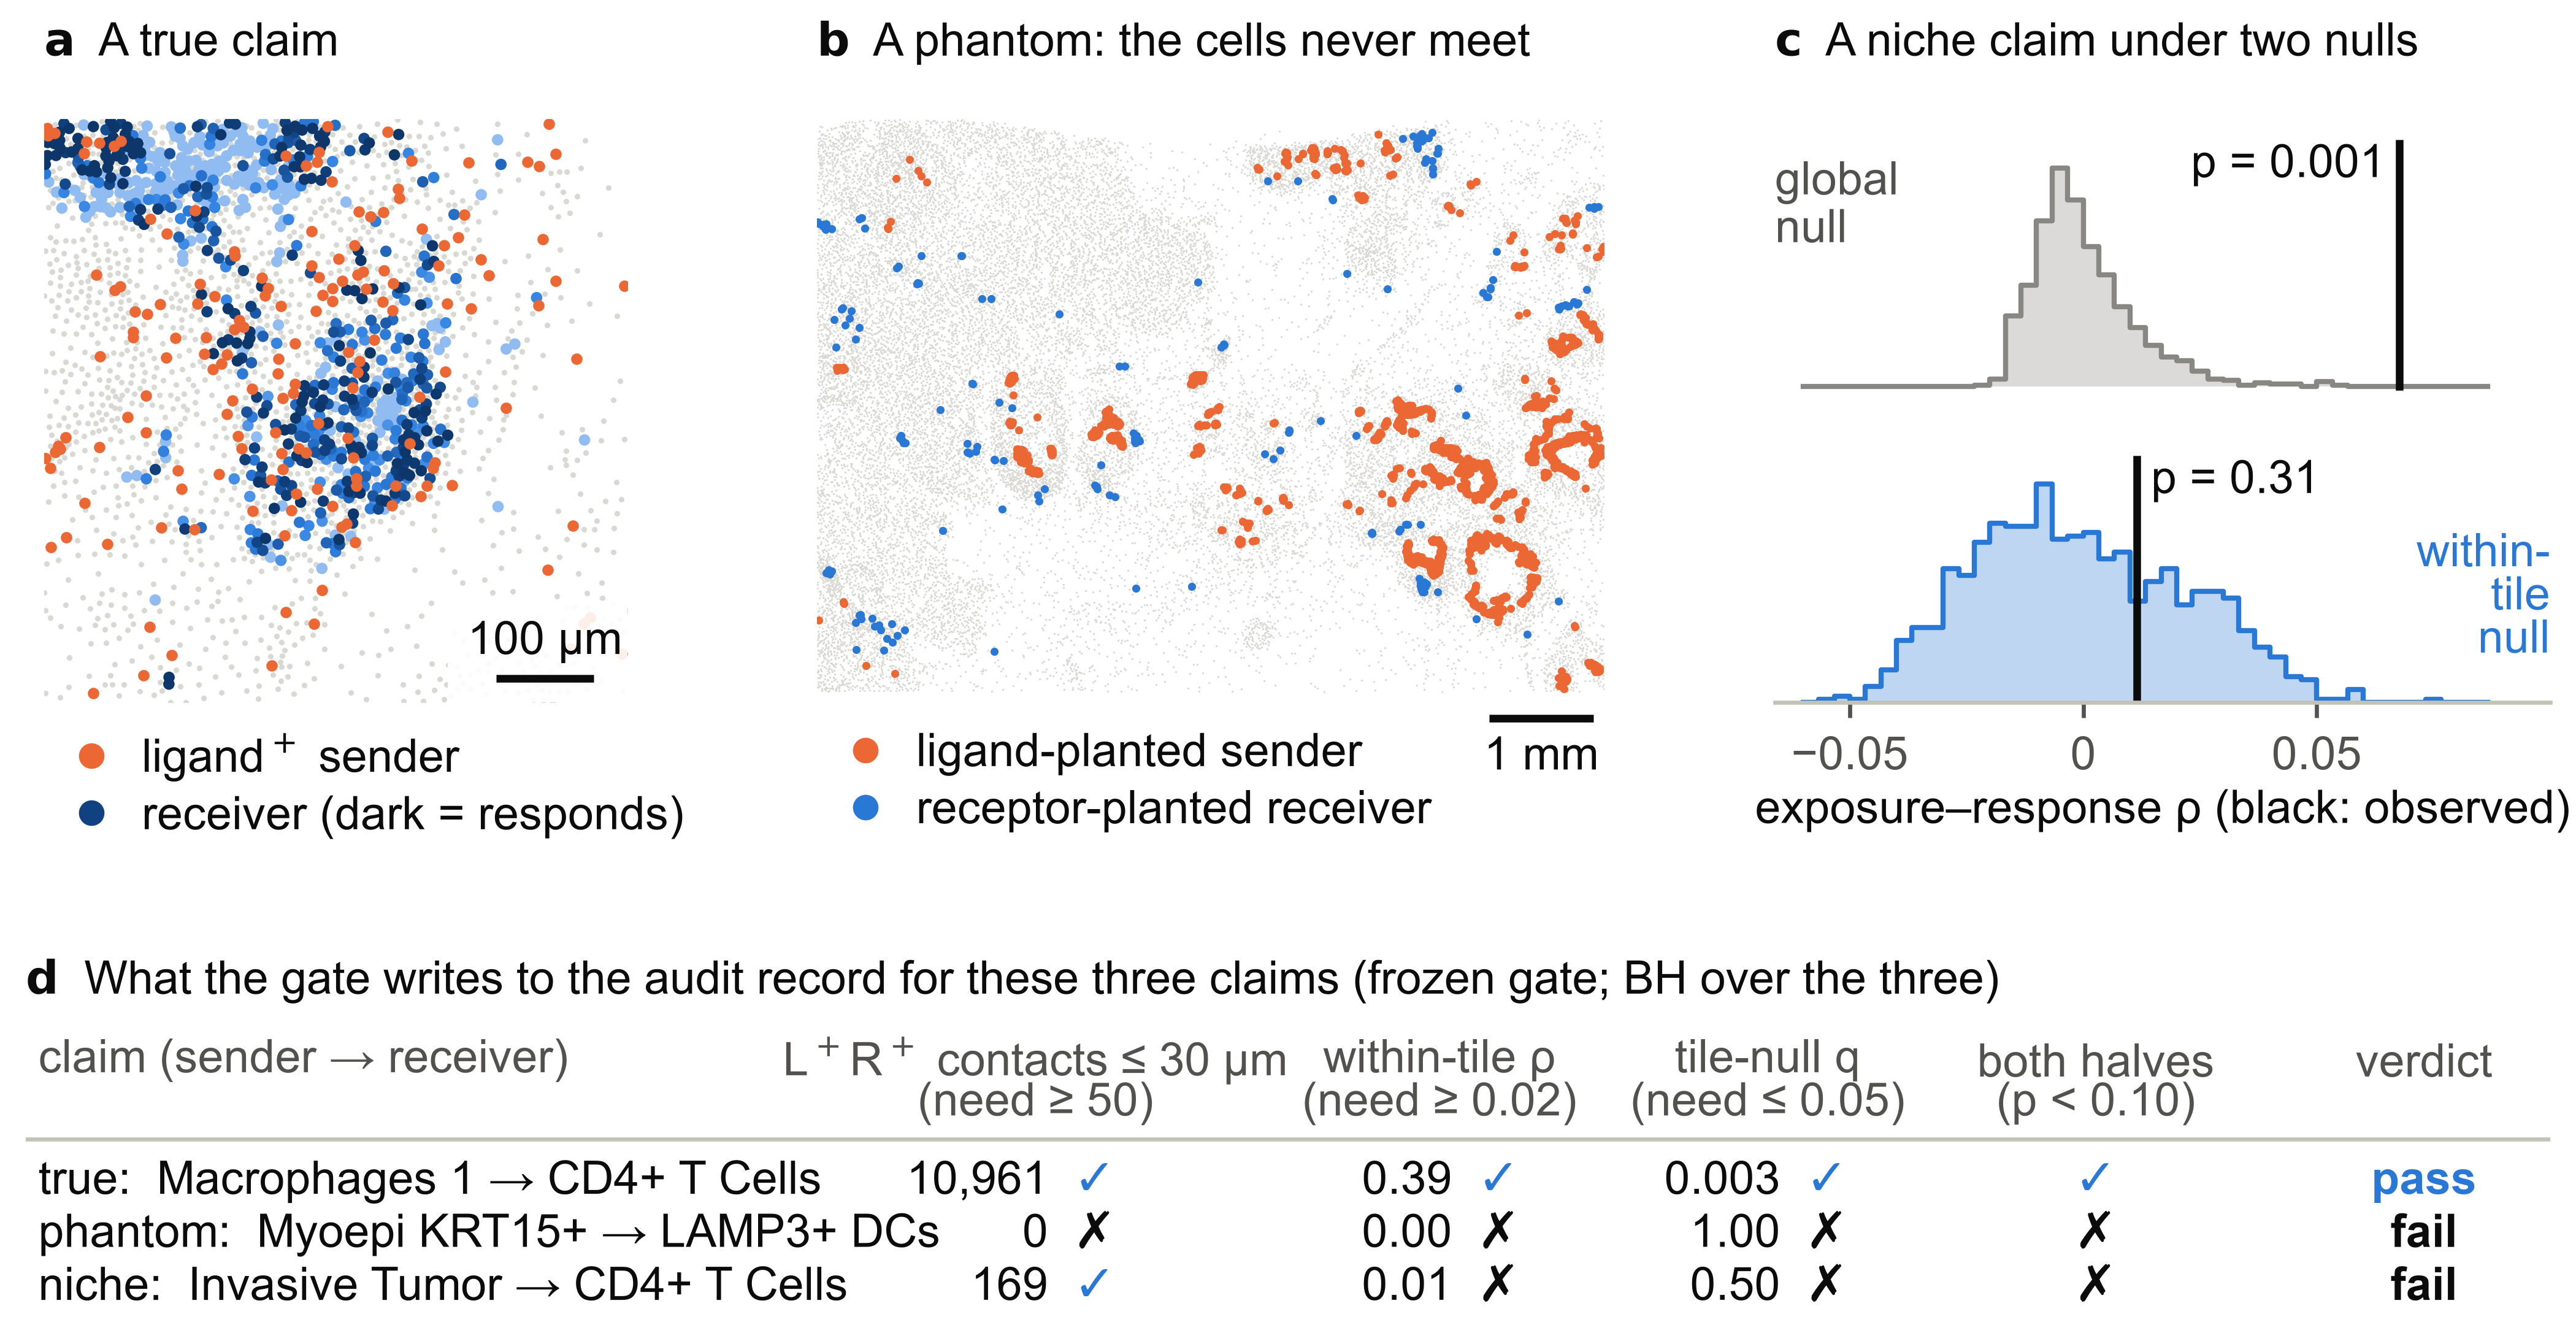
\includegraphics[width=\textwidth]{figures/fig1_overview.png}
\caption{The claim gate on a real tissue state: breast Rep1 with one benchmark instance planted (dev seed 0, used for
illustration only). (a) A planted true claim in a 600\um\ window: receivers near ligand$^+$ senders respond. (b) A
planted phantom: ligand and receptor rise in cells that never come within contact range. (c) A niche-confounded claim
looks significant under a global permutation null but not under the gate's within-tile null (nulls redrawn for
display, 1,000 permutations each). (d) The gate's four checks for the three claims, as written to the audit record.}
\label{fig:overview}
\end{figure*}

\section{Experimental Design}
\paragraph{Two pre-registered phases.} In Phase~1 we fixed hypotheses H1--H3, metrics, verdict rules and data splits in
a version-controlled document before any evaluation. We tuned the gate on dev seeds 0--4 of breast Rep1 and froze it;
the configuration chosen equalled the pre-registered defaults. Test data (seeds 100--104 on all four sections) were run
once. Phase~2, a later amendment (Amendment~4), added hypotheses H4--H7 and a new confirmatory seed set, N2 (seeds
200--209), never used for tuning or for Phase~1. The gate stayed frozen. This paper reports H1--H5; H6 (enforced gating
for agents) and H7 (real-data positive controls) are still being evaluated. Analyses not named in the pre-registration
are labelled exploratory, and the Appendix lists all amendments, including a disclosure about the timestamp of
Amendment~4.
% LANE-C/E PENDING (lane L): add H6 and H7 here, to Table 1 and to Results when lanes E and C report.

\paragraph{Conditions and metrics.} We use two expression-only tools: a CellPhoneDB-style mean score with 1,000 label
permutations (\emph{cpdb}) and a LIANA/CellChat-style product score (\emph{prod}). Phase~1 also ran tool-using LLM
agents (\texttt{gemini-2.5-flash} and \texttt{deepseek-flash}) asked for the top-10 interactions with evidence, with and
without the gate available as a \texttt{verify\_claim} tool. The \emph{phantom rate} of a list is the share of its claims
that are not planted-true; every non-true claim counts, whatever its kind. \emph{Retention} is the share of the list's
true claims that pass the gate, and the \emph{post-gate phantom rate} is the non-true share of the claims that pass.
Confidence intervals (95\%) come from a hierarchical bootstrap over (tissue, seed) units and then claims. Phase~2 pools
the top-10 lists of both tools over four tissues and ten N2 seeds: 80 lists and 800 claims per condition.

\paragraph{H4: misspecified mechanisms.} We re-planted the targets of true pairs with mechanisms the gate does not
assume and left every other channel untouched, so that variants differ only in how receivers respond. A1 uses a ring
kernel (15--30\um). A2 uses half or double the gate's range (15 or 60\um). A3 is diffusive paracrine signalling with an
80\um\ range and a 40\um\ decay length, the scale measured for cytokine communication in vivo \cite{oyleryaniv2017}.
In A4 the receptor is bound but no target responds. A5 mixes A1--A4 within each tissue and adds two kinds of hard
negative: \emph{decoy senders}, a second cell type that also expresses the true ligand but does not signal, and
stronger niche-confounded pairs that reach the top-10. A0 is the gate-matched reference. H4 holds if retention
$\geq0.60$ and post-gate phantom rate $\leq0.10$ in at least four of the five variants (A2 counts once, and both of its
ranges must pass). It is falsified if retention falls below 0.50, or the phantom rate exceeds 0.15, in at least two.

\paragraph{H5: weaker signals.} Effect levels of 1, 1/2, 1/4 and 1/8 scale the planted means of every planted
category. H5 holds if the expression-only phantom rate rises as the effect falls (median Spearman $\rho\leq-0.80$
across levels over 40 tissue--seed units) and the post-gate phantom rate stays $\leq0.15$ at every level. It is
falsified if $\rho>-0.50$ or the post-gate rate exceeds 0.20 at any level.

\begin{table*}[t]
\centering
\small
\begin{tabular}{@{}lp{6.3cm}p{5.4cm}l@{}}
\toprule
 & Pre-registered criterion & Outcome & Verdict \\
\midrule
H1 & Expression-only tools and unguided agents report $\geq$30\% phantoms at $K{=}10$ (CI lower bound $\geq$0.20)
   & dev \devBreastReponeProdKTenPR{}--\devBreastReponeCpdbKTenPR{}; held-out tools
     \testPancreasCpdbKTenPR{}--\testBreastReponeCpdbKTenPR{}; agents \agTestAllBothPR{}
   & not supported \\
H2 & The gate cuts the phantom rate by $\geq$50\% and keeps $\geq$80\% of true claims
   & no phantom left after gating in any list set; retention $\geq$\agDevBreastReponeGeminiRet{}
   & supported \\
H3 & H2 holds without retuning on held-out breast seeds and $\geq$2 other tissues
   & held-out breast Rep1 and Rep2, pancreas, lung
   & supported \\
H4 & Retention $\geq$0.60 and post-gate phantom rate $\leq$0.10 in $\geq$4 of 5 misspecified variants (N2)
   & \hfourNmet{} of 5; A4 retention \hfourAfourRet{}, A5 post-gate phantom rate \hfourAfivePRafter{}
   & \textbf{not met} \\
H5 & Expression-only phantom rate rises as effect falls (median $\rho\leq-0.80$); post-gate rate $\leq$0.15 at every
     level (N2)
   & median $\rho=$ \hfiveMedRho{}; post-gate rate \hfiveDefaultEighthPRafter{} at effect 1/8
   & \textbf{falsified} \\
\bottomrule
\end{tabular}
\caption{Pre-registered hypotheses and outcomes. H1--H3 are Phase~1 (test seeds 100--104), H4--H5 Phase~2 (fresh
seeds 200--209); all at $K{=}10$ with the frozen gate. H1 was inconclusive for most conditions and falsified for three
agent conditions on held-out tissues. H4's formal category under the pre-registered rules is \emph{inconclusive} (one
variant fails each criterion, and falsification needs two failing the same one); it is a miss. Per-condition Phase~1
results: Appendix Table~\ref{tab:verdicts}.}
\label{tab:hyp}
\end{table*}

\section{Results}
\subsection{Phase 1: The Gate Removes Easy Phantoms}
Expression-only tools did produce phantoms, but fewer than we expected. Their dev top-10 lists were
\devBreastReponeCpdbKTenPR{} (cpdb) and \devBreastReponeProdKTenPR{} (prod) phantom, held-out lists
\testPancreasCpdbKTenPR{}--\testBreastReponeCpdbKTenPR{}, and LLM agents with spatial tools
\agTestAllBothPR{} \agTestAllBothPRci{} over \agTestAllBothRuns{} held-out runs. None reached the pre-registered 0.30,
so H1 is not supported (Table~\ref{tab:hyp}). One reason is that ranking by log-normalised type means favours true
plants over matched decoys, because a decoy concentrates the same count increase in fewer cells.

The gate itself did what H2 and H3 ask. It removed every phantom from the expression-only top-10 lists on dev and on
every held-out set, including a second breast section and pancreatic and lung cancer, whose panel and annotation differ
from the breast data it was tuned on, and it kept at least \agDevBreastReponeGeminiRet{} of the true claims (Appendix
Figure~\ref{fig:phase1}). Gating the agents' lists after the fact left a phantom rate of \agTestAllBothPRafter{}, with
retention \agTestAllBothRet{}. Agents that had the gate as a tool did worse. Their held-out phantom rate was
\agTestAllBothToolPR{} \agTestAllBothToolPRci{}, and \compTestVerifiedFailSubmitted{} of \compTestSubmitted{} submitted
claims had been rejected by the agent's own \texttt{verify\_claim} call; another \compTestUnverified{} were never
checked. Several transcripts describe a claim as lacking spatial support and submit it anyway to fill the requested ten.

Two checks went beyond planted phantoms. On \rnullN{} random claims built from real panel genes in real breast tissue,
\rnullFrozenFive{} reached $p<0.05$ under the gate's tile-restricted null and \rnullNoTilesFive{} under a global one, so
the tile restriction matters for calibration on real data. On real breast tissue, where the receptor is the only
readout available, the gate passed \realPdlPass{} of the \realPdlN{} PD-L1/PD-1 claims that an expression tool ranked
highest. The ligand- and receptor-positive cells had too few contacts, at chance level (Appendix
Figure~\ref{fig:pdl1}). It also passed \realPosctlPass{} of \realPosctlN{} contact-dependent positive controls. Without
a target readout the gate cannot certify a real positive, a limit that Phase~2 made precise.

A caveat bounds all of this. The phantoms in these lists carry no target response, so any response check rejects them,
and the default top-10 lists hardly contain the hard negatives: across Phase~1 tool lists, \compTenNiche{} of
\compTenN{} claims were niche-confounded. Phase~1 shows that the gate does its basic job. It does not show that the gate
is hard to fool.

\begin{figure*}[t]
\centering
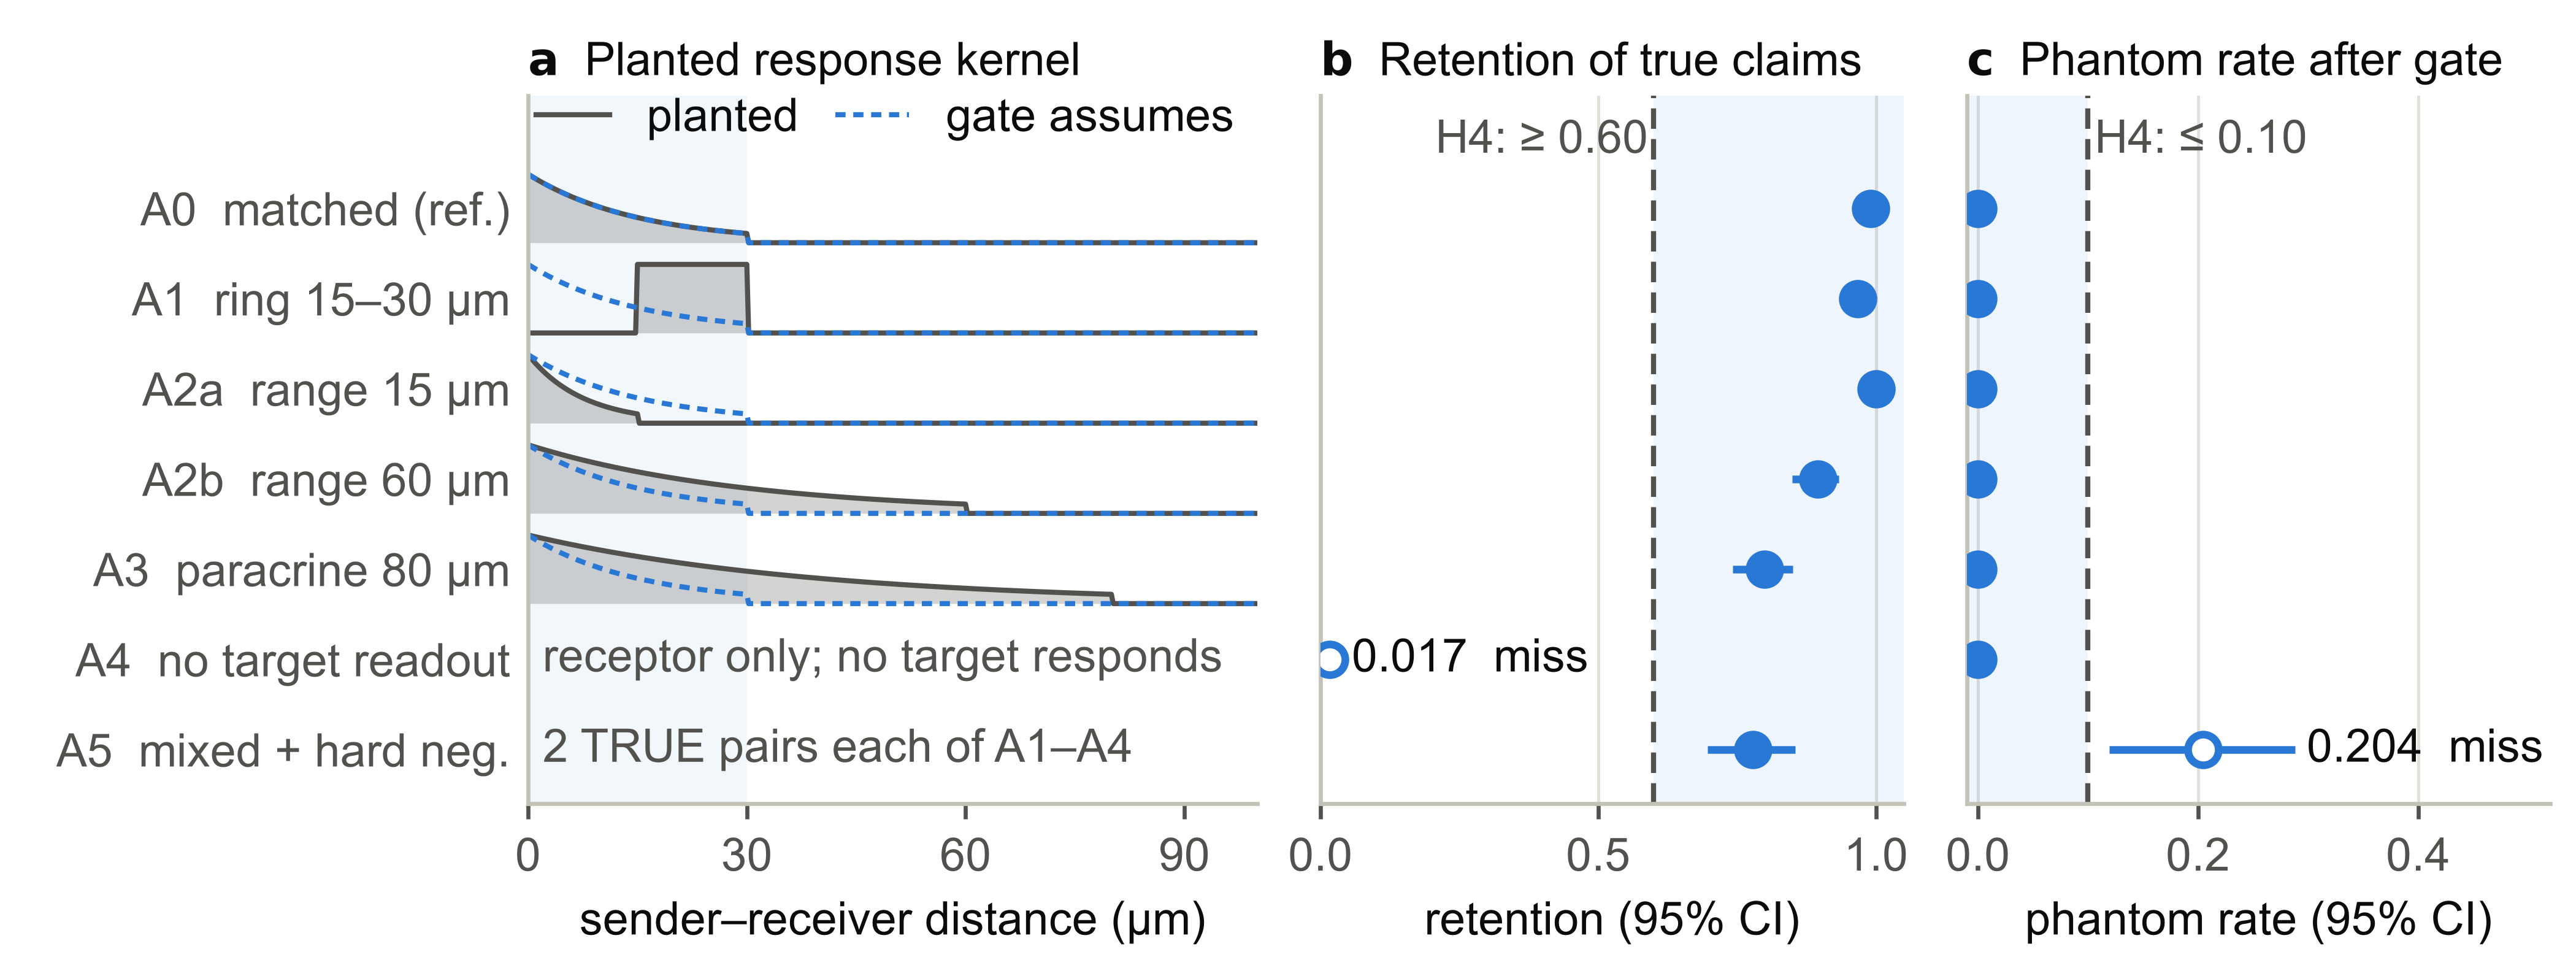
\includegraphics[width=\textwidth]{figures/fig2_h4_misspecification.png}
\caption{H4 on fresh seeds (N2: ten seeds $\times$ four tissues, $K{=}10$, cpdb and prod pooled). (a) The planted
response kernel of each variant (grey) against the kernel the gate assumes (dashed blue); the shaded band is the
gate's 30\um\ window. (b) Retention of true claims and (c) post-gate phantom rate, with 95\% CIs and the pre-registered
thresholds. Filled markers meet the variant's criterion. Three of five variants meet both criteria (A2 needs both
ranges); four were required.}
\label{fig:h4}
\end{figure*}

\subsection{H4: Misspecified Mechanisms}
The gate tolerated getting the shape and range of the mechanism wrong (Figure~\ref{fig:h4}). Retention was
\hfourAoneRet{} with a ring kernel, \hfourAtwoaRet{} with a 15\um\ range, \hfourAtwobRet{} with a 60\um\ range and
\hfourAthreeRet{} with 80\um\ paracrine signalling, against \hfourAzeroRet{} for the matched reference. Retention falls
as the true range outgrows the gate's 30\um\ window, and the losses are all of one kind. Every true claim the gate
dropped in A2b and A3 failed split-half replication (\hfourFailAthreeSplitInconsistent{} of
\hfourFailAthreeNTrueFailed{} in A3). Long-range signals saturate the response inside the window, so the within-tile
gradient that the gate looks for flattens.

Two variants failed, one more than H4 allows. With no responding target (A4), the gate kept \hfourAfourRet{}
\hfourAfourRetci{} of true claims. We predicted this before seeing the data, and it is not a bug: the gate looks for a
response, and A4 has none. With mixed mechanisms and hard negatives (A5), retention was acceptable (\hfourAfiveRet{}),
but \hfourAfivePRafter{} \hfourAfivePRafterci{} of the passed claims were false: \hfourAfiveFalseTotal{} of
\hfourAfiveNpass{} passes, \hfourAfiveFalseNiche{} of them hard-niche and \hfourAfiveFalseDecoy{} decoy-sender claims.
The miss is smallest in breast Rep1, the tuning tissue, where the rate (\hfourAfivePRafterBreastRepone{}) stays under
the threshold, and largest in lung (\hfourAfivePRafterLung{}; every tissue is shown in Figure~\ref{fig:pertissue}).
Three of five variants met both criteria where four were required, so \textbf{H4 is
not met}. The formal category under our rules is inconclusive rather than falsified, because falsification needs two
variants failing the same criterion and here one fails each. We read it as a miss, not a partial success.

The zero post-gate phantom rates of A0--A4 say little, by construction. Those variants share the default lists, which
over 80 lists held \hfourCompAzeroTrue{} true, \hfourCompAzeroPhantom{} phantom, \hfourCompAzeroOther{} wrong-type-pair
and \hfourCompAzeroNiche{} niche-confounded claims. A5 is the only H4 variant whose lists contain negatives that can
pass, and it is the one that failed. Its high expression-only phantom rate (\hfourAfivePR{}) is also built in, since we
strengthened the hard negatives until they reached the lists.

\begin{figure*}[t]
\centering
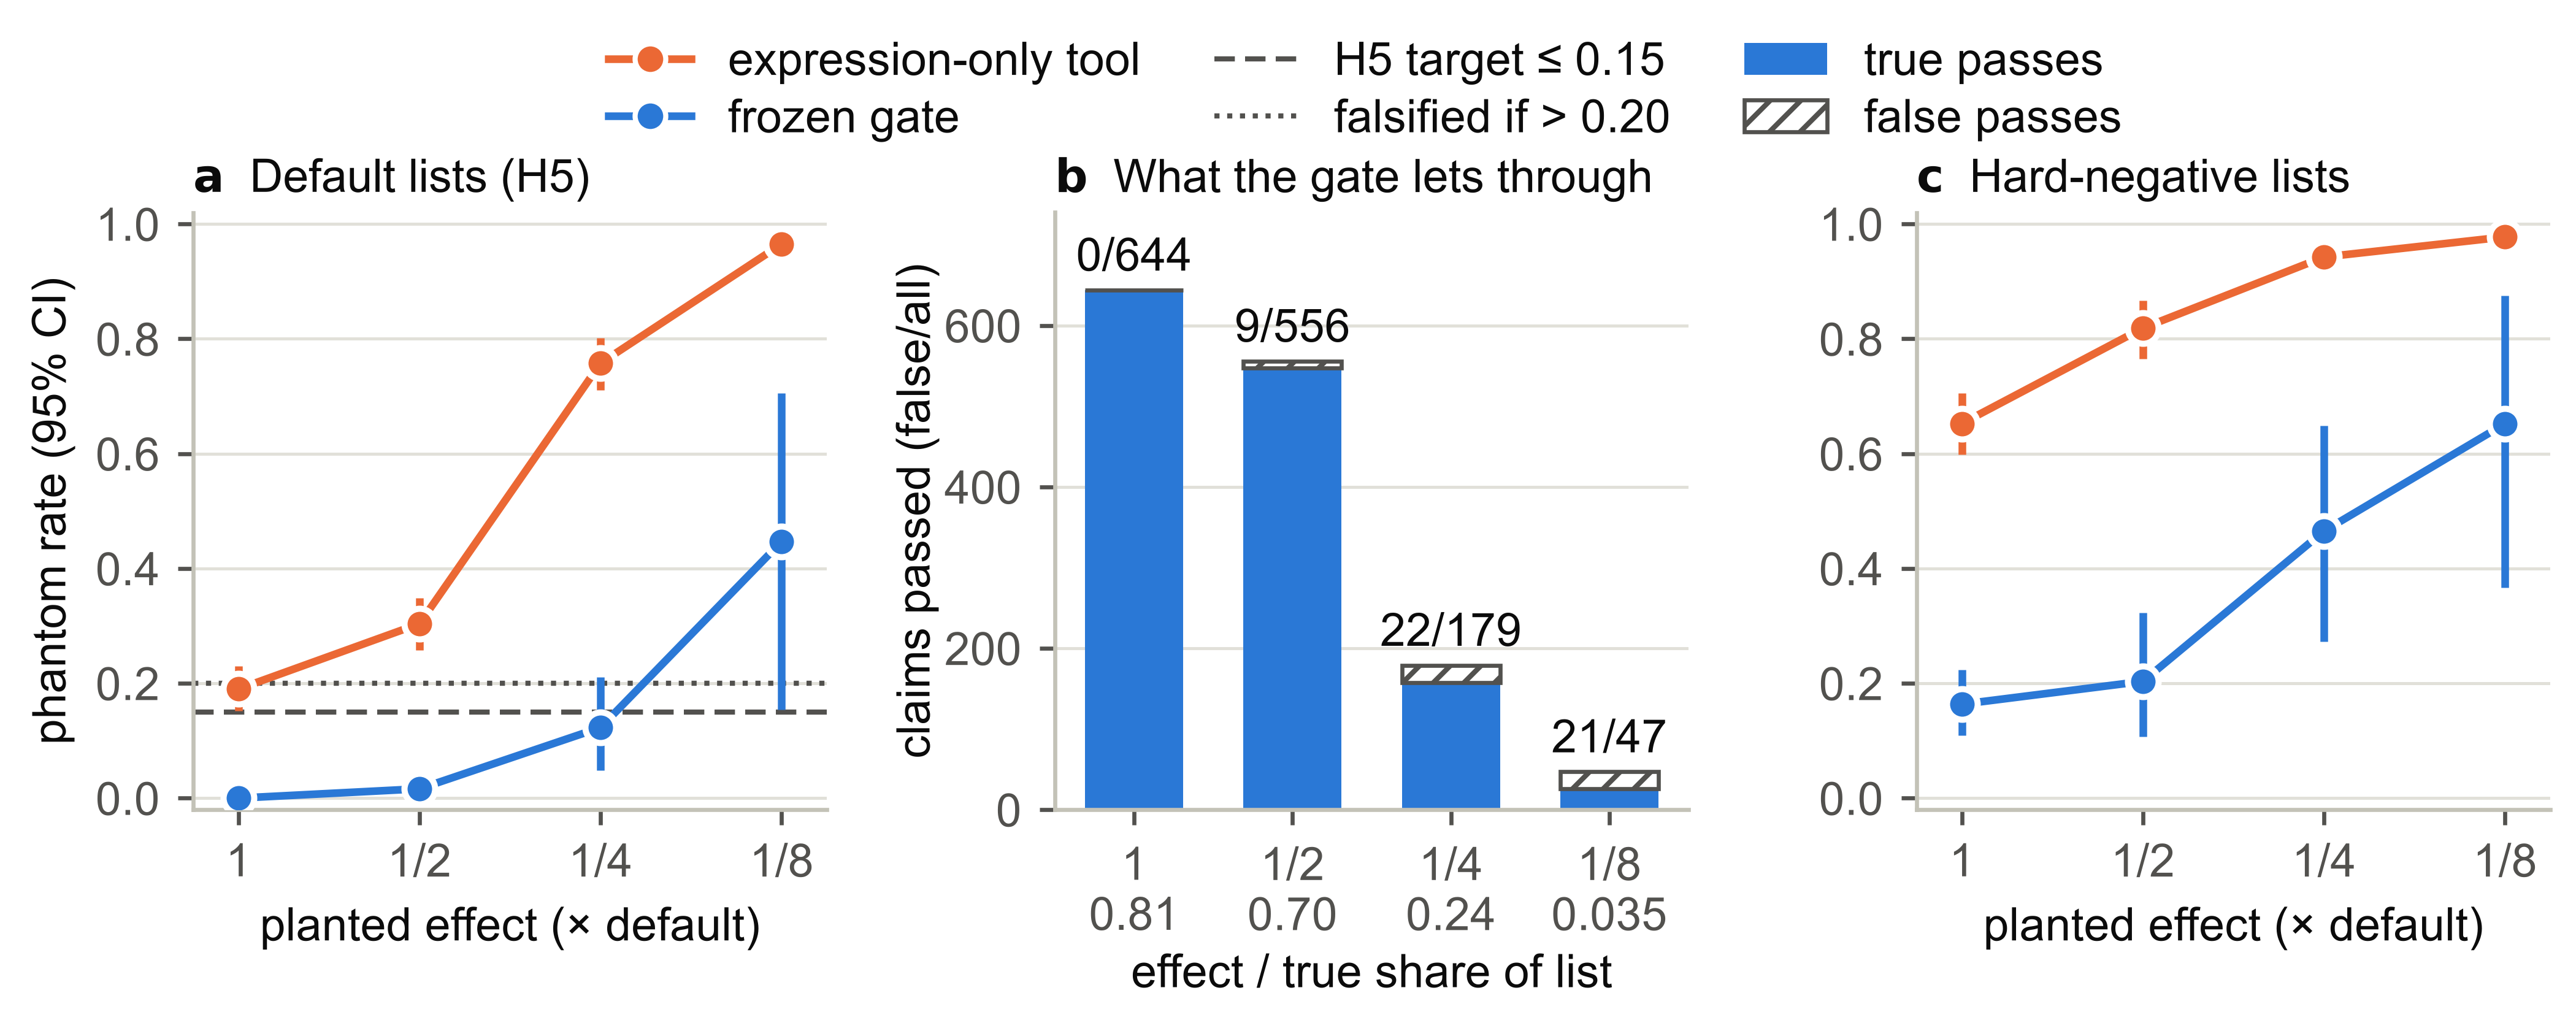
\includegraphics[width=\textwidth]{figures/fig3_h5_dose_response.png}
\caption{H5 on fresh seeds (40 tissue--seed units, $K{=}10$, cpdb and prod pooled, 95\% CIs). (a) Phantom rate of
expression-only lists before and after the frozen gate as the planted effect falls. (b) What the gate passed at each
level: true passes and false passes (labels: false/all), with the true share of the lists under each effect level.
(c) The same as (a) for exploratory hard-negative lists (gate-matched true response plus the decoy senders and hard
niche pairs of A5).}
\label{fig:h5}
\end{figure*}

\subsection{H5: Weaker Signals}
Weakening the planted effect hurt the expression-only tools exactly as predicted (Figure~\ref{fig:h5}a). Their phantom
rate rose from \hfiveDefaultOnePR{} at full effect to \hfiveDefaultEighthPR{} at one eighth; the median per-unit
Spearman $\rho$ was \hfiveMedRho{}, and all \hfiveNunitsLe{} units were at or below $-0.80$. The gate held at half
effect (\hfiveDefaultHalfPRafter{}) and, narrowly, at a quarter (\hfiveDefaultQuarterPRafter{}
\hfiveDefaultQuarterPRafterci{}). At one eighth, \hfiveDefaultEighthPRafter{} \hfiveDefaultEighthPRafterci{} of what
it passed was false, above both the 0.15 target and the 0.20 line. \textbf{H5 is falsified.}

The more useful finding is why. The gate did not get worse per claim. The share of negatives it let through stayed low
and roughly flat: \baseHalfNegPassRate{} at 1/2, \baseQuarterNegPassRate{} at 1/4 and \baseEighthNegPassRate{} at 1/8.
What collapsed was the list it was given. The true share of the expression-only lists fell from
\baseOnePrevalenceTrue{} to \baseEighthPrevalenceTrue{}, and with only \hfiveDefaultEighthNtrue{} true claims among 800,
a negative pass rate of \baseEighthNegPassRate{} is enough to make \baseEighthNegPassed{} of \hfiveDefaultEighthNpass{} passes
false (Figure~\ref{fig:h5}b). This is the base-rate effect familiar from the false-discovery literature: whether a
positive finding is true depends on the share of true relationships among those tested, not only on the test
\cite{ioannidis2005}. The one-eighth estimate rests on \hfiveDefaultEighthNpass{} passes and varies across tissues,
from \hfiveEighthPRafterPancreas{} in pancreas to \hfiveEighthPRafterBreastRepone{} in breast Rep1
(Figure~\ref{fig:pertissue}c), but the mechanism behind it does not depend on that spread. Hard-negative lists (exploratory) show the same pattern from a worse start:
\hfiveAfivemOnePRafter{} of passes were false at full effect and \hfiveAfivemEighthPRafter{} at one eighth
(Figure~\ref{fig:h5}c).

\begin{figure*}[t]
\centering
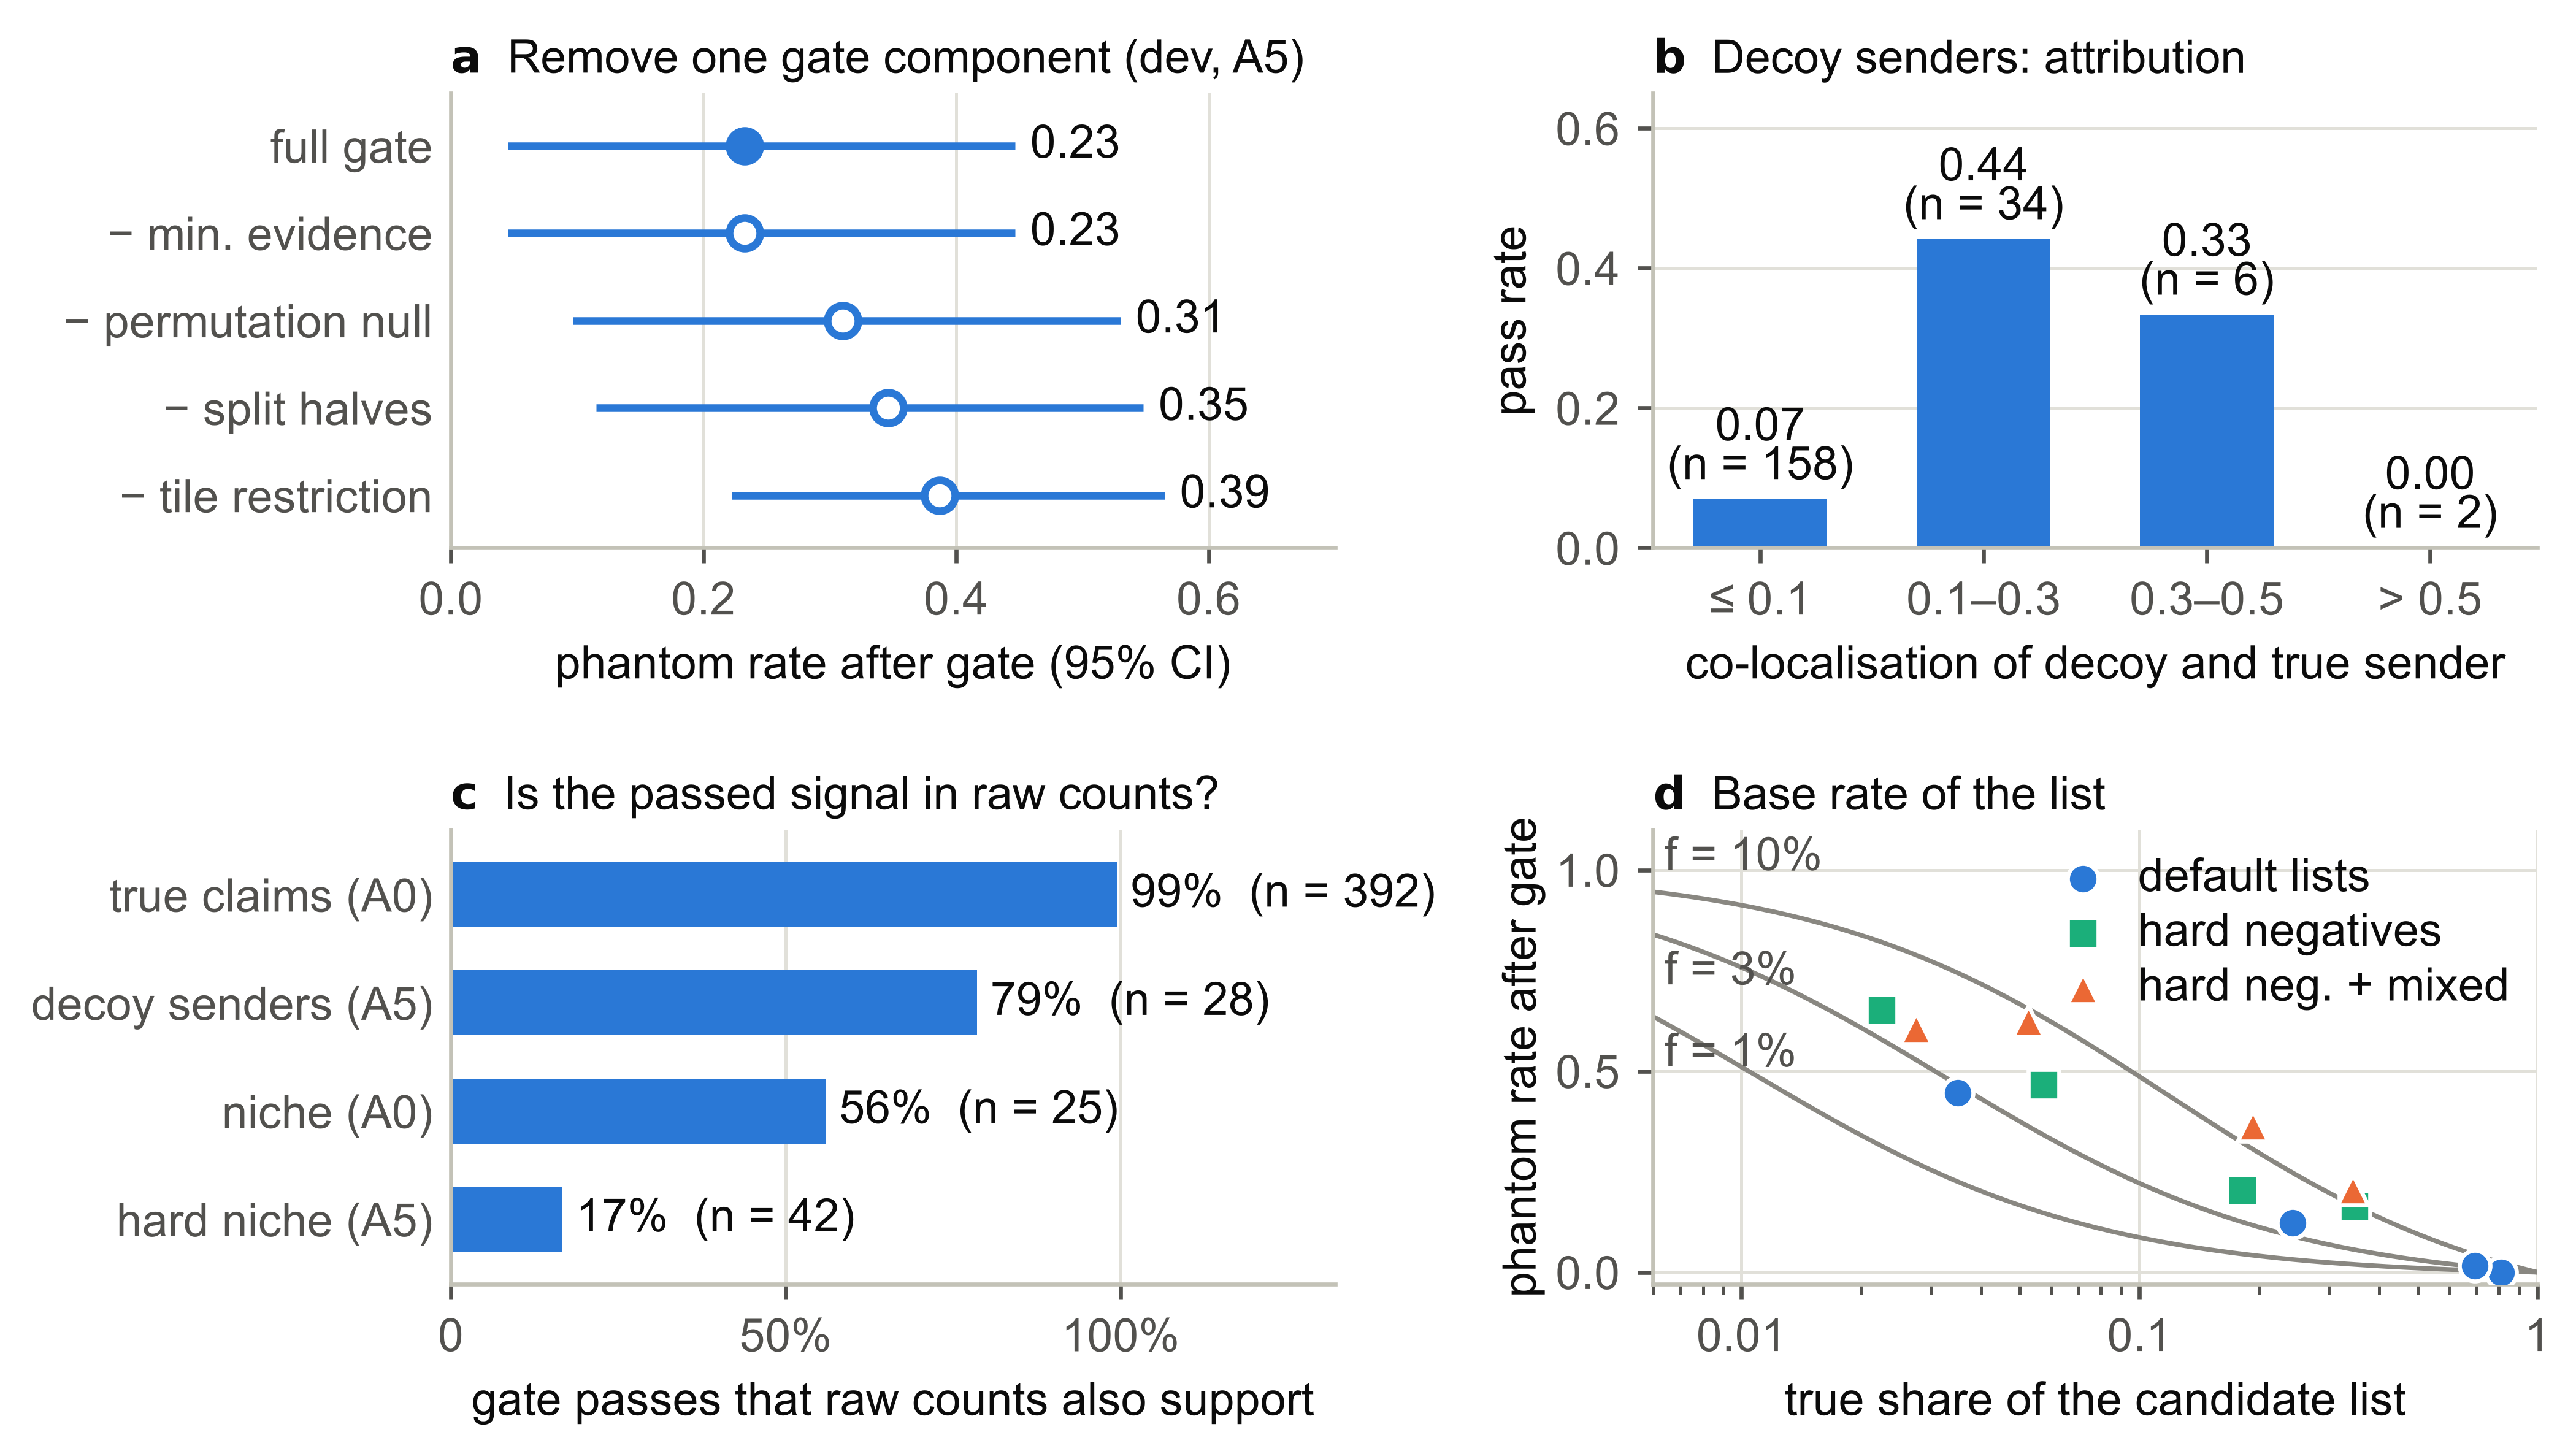
\includegraphics[width=\textwidth]{figures/fig4_failure_map.png}
\caption{Failure map (exploratory analyses of the frozen gate). (a) Post-gate phantom rate on A5 lists with one gate
component removed at a time (dev seeds 0--4, breast Rep1). (b) Pass rate of decoy-sender claims by the co-localisation
of decoy and true sender (correlation of their exposures across receivers; N2). (c) Share of gate passes whose signal
is also supported by raw counts (N2). (d) Post-gate phantom rate against the true share of the candidate list, for
default and hard-negative lists at all four effect levels (N2). Grey curves: the expected rate for a gate that keeps
95\% of true claims and passes a fraction $f$ of negatives.}
\label{fig:failure}
\end{figure*}

\subsection{A Failure Map}
Together, the misses point to four distinct ways in which the gate fails (Figure~\ref{fig:failure}). Each has a
mechanism we can name. We fixed none of them: the gate stays frozen, and any change would need fresh seeds and a new
amendment.

\paragraph{No readout, no detection.} The gate tests whether exposure predicts a response. Signalling that changes no
measured transcript is invisible to it, as in A4, where retention was \hfourAfourRet{}. Removing the permutation test
lifts this to \ablAfourRetNoPerm{} on dev seeds, but those extra passes have no planted response behind them; the
permutation null is what keeps unsupported claims out. On real tissue with small panels, where target genes are often
unmeasured, this is the common case. Only \lrBreastRepone{} of \lrConsensus{} consensus ligand--receptor pairs are
measurable on the breast panel, and missing readouts are why the gate failed every real positive control.

\paragraph{Co-localised senders.} A decoy sender expresses the true ligand but does not signal. When its cells sit
apart from the true sender's, the gate rejects it: the pass rate was \decoyPassLow{} ($n=\decoyNLow{}$). When the two
exposures overlap (co-localisation 0.1--0.3), the pass rate rises to \decoyPassMid{} ($n=\decoyNMid{}$;
Figure~\ref{fig:failure}b). The response is real, since \rawSupDecoy{} of passed decoys are also supported by raw
counts, but it is attributed to the wrong sender. A correlational test cannot tell apart senders that occupy the same
neighbourhoods. Conditioning on the exposure from the other ligand-expressing types would.

\paragraph{Normalisation and density.} The gate normalises each cell's counts by its library size. In these sections
library size correlates with local cell density, with a sign that depends on the tissue: Spearman $\rho$ with the number
of cells within 30\um\ was \libDensBreastRepone{} and \libDensBreastReptwo{} in the two breast sections,
\libDensLung{} in lung and \libDensPancreas{} in pancreas (Figure~\ref{fig:libsize}). The normalisation factor can
therefore co-vary with exposure.
Only \rawSupNicheHard{} of hard-niche passes are supported by raw counts, against \rawSupTrue{} of true passes
(Figure~\ref{fig:failure}c), and the share is low in every tissue, from \normNicheRawBreastReptwo{} in breast Rep2 to
\normNicheRawPancreas{} in pancreas, where library size and density correlate positively. This matches reports that library size carries tissue structure \cite{bhuva2024} and that
count-based normalisation creates region-specific false positives in imaging-based data \cite{atta2024}. Normalising by
cell area, or permuting within density strata, are the obvious candidates to test.

\paragraph{The base rate of the list.} A per-claim filter can reject most negatives and still return a list that is
mostly false if the list it was given was mostly false (Figure~\ref{fig:failure}d). The observed points follow the
expected curves: what moves them up is the true share of the list, not a change in the gate.

\paragraph{Which components do the work.} On hard-negative lists (dev seeds, exploratory), no single component is
enough (Figure~\ref{fig:failure}a). Removing the tile restriction raised the post-gate phantom rate from
\ablAfiveFull{} to \ablAfiveNoTiles{}, removing split-half replication raised it to \ablAfiveNoSplit{}, and removing
the permutation null raised it to \ablAfiveNoPerm{}; the minimum-evidence rule made no difference (\ablAfiveNoMinEvidence{}).

\begin{figure*}[t]
\centering
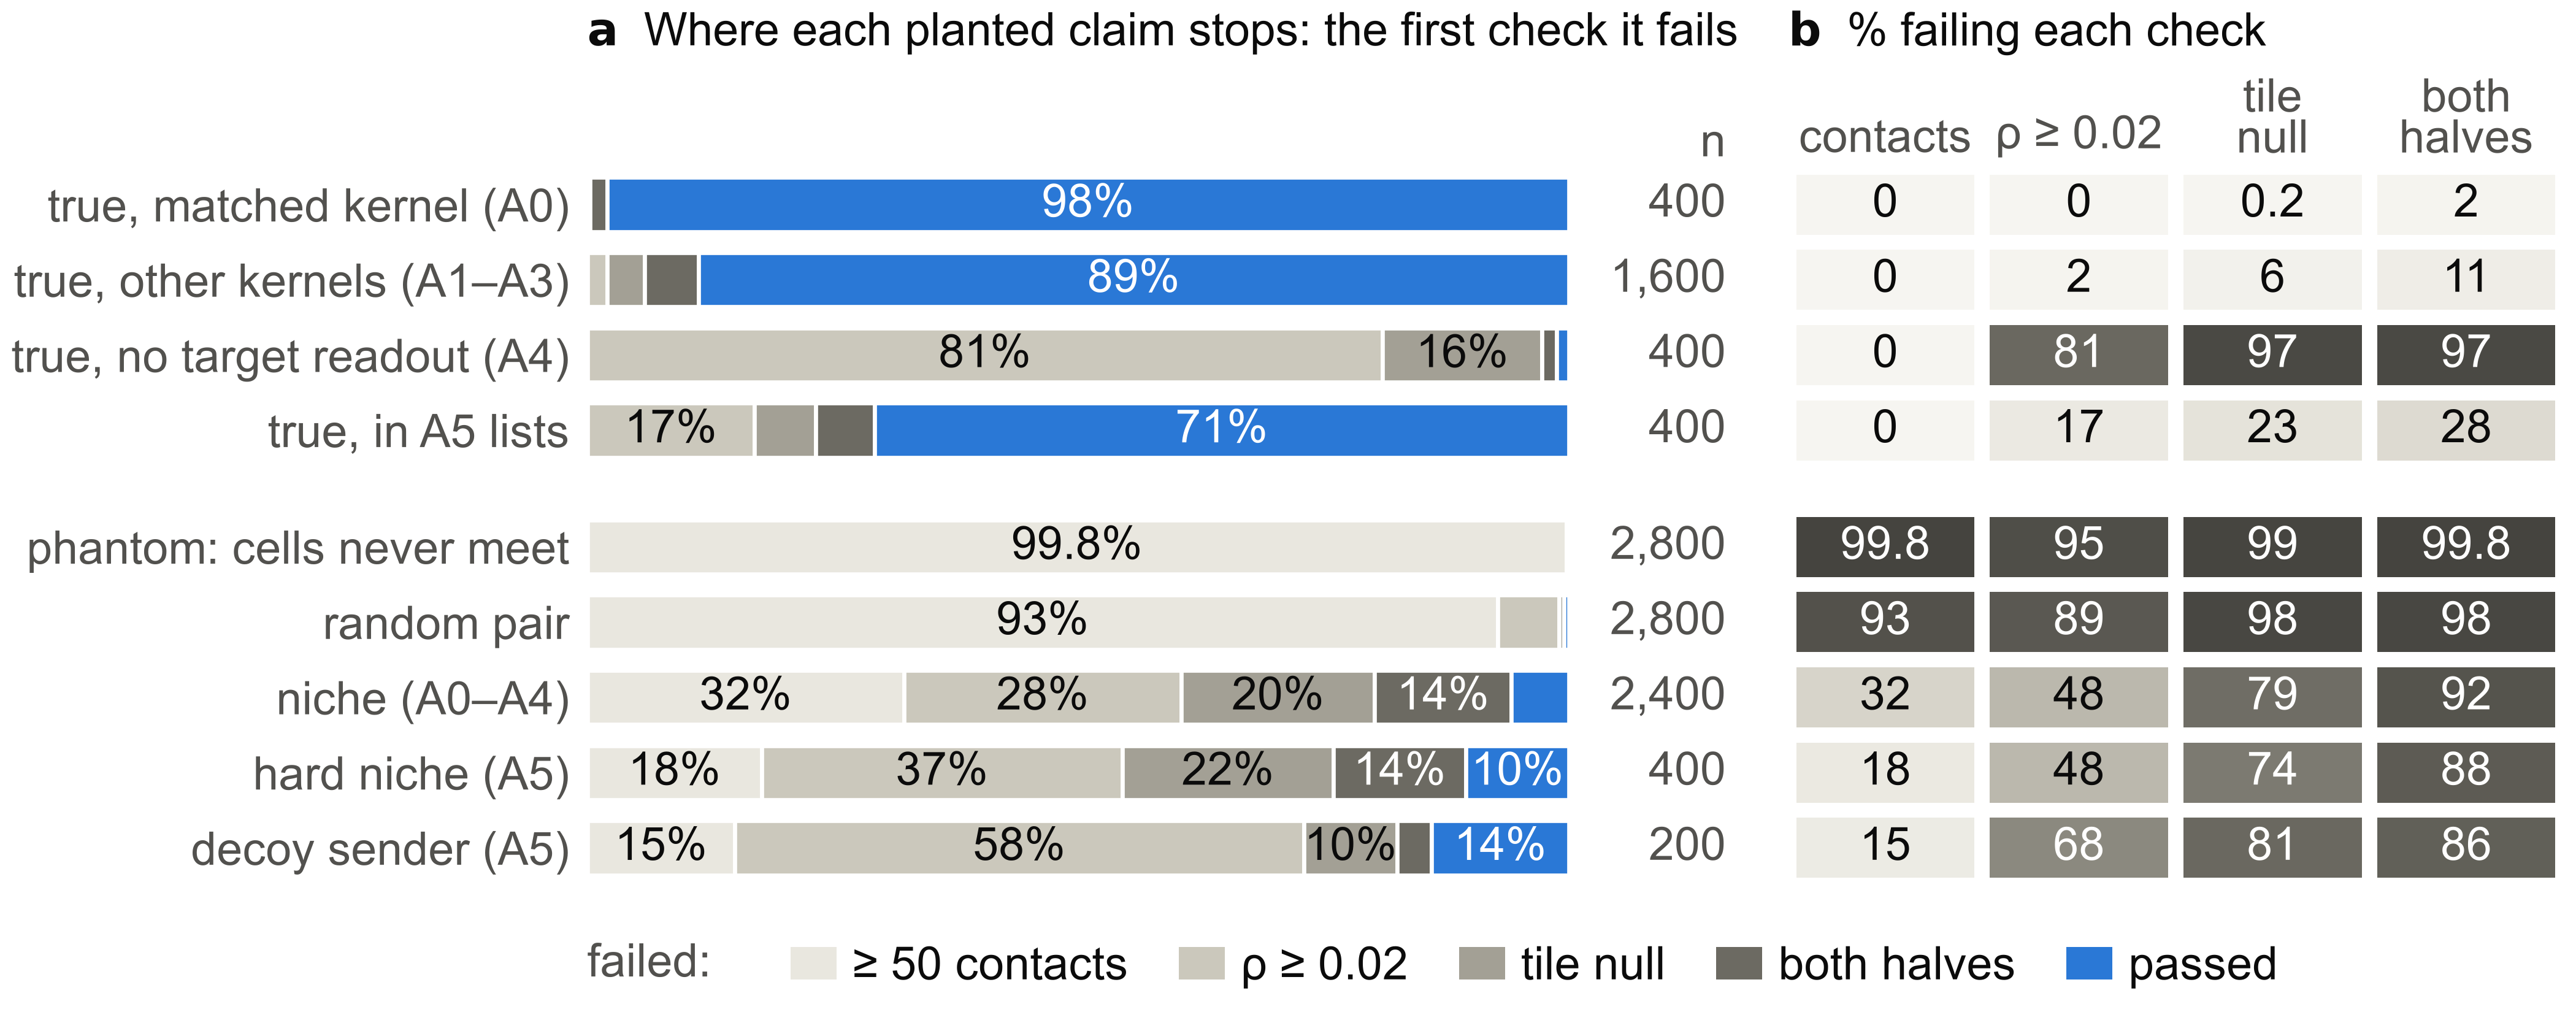
\includegraphics[width=\textwidth]{figures/fig5_claim_fate.png}
\caption{Where each planted claim stops (frozen gate on fresh seeds: 4 tissues, seeds 200--209, variants A0--A5;
\fateNplanted{} planted claims, all planted claims of an instance gated as one list). This is a description of the
committed decisions; nothing was re-run. (a) The first check each claim fails, taking the checks in the order shown;
the gate itself applies all four and passes a claim only if none fails. Blue: passed. (b) Percentage of claims that
fail each check; a claim can fail several.}
\label{fig:fate}
\end{figure*}

\paragraph{Which check stops which claim.} The ablations remove a component and rerun the gate on dev seeds. The
committed decisions on fresh seeds tell the same story without a rerun (Figure~\ref{fig:fate}), and they show that each
kind of false claim meets a different check. Phantoms fall at the first one: \fatePhantomFirstContacts{} have too few
contacts between ligand- and receptor-expressing cells, because their cells never meet. Most random pairs fall there
too (\fateRandomFirstContacts{}). Niche claims are the hard case, and they are spread over all four checks. For
\fateNicheOnlyHalves{} of them split-half replication is the only check they fail, so without it they would pass.
That protection has a price: replication is also the only check failed by \fateTrueAoneathreeOnlyHalves{} of the true
claims planted with the wrong kernel (A1--A3). True claims with no responding target (A4) stop mostly at the effect
threshold (\fateTrueAfourFirstEffect{}), the readout problem seen from inside the gate. What gets through is what the
failure map predicts: \fateNicheHardPassRate{} of hard-niche claims and \fateDecoySenderPassRate{} of decoy senders.

\section{Discussion}
\paragraph{What a verifier should report.} A verification layer for a medical world model is useful only if its limits
travel with its verdicts. Our results suggest four things an audit record should state next to each pass or fail:
whether a response readout exists for the claim; whether other candidate senders share the claimed sender's
neighbourhood; how the response was normalised; and how many true claims the candidate list could plausibly contain.
The last point is the least obvious. A gate that is excellent claim by claim can still hand a clinician a list that is
half wrong, and nothing in the per-claim verdicts would show it. In a decision-support setting, for example when asking
whether PD-1/PD-L1 blockade has a cellular substrate in a tumour, the honest output of the gate is often ``no evidence
either way'', and the record should say so.

\paragraph{What we would test next.} Each failure suggests a fix, and each fix needs its own pre-registered test on seeds
the gate has never seen, because tuning on the seeds reported here would turn our misses into overfitting.
Co-localised decoys call for \emph{sender conditioning}: test the claimed sender's partial effect given the exposure
from every other ligand-expressing type. The normalisation confound calls for \emph{a density-aware response model}
with library size or cell area and local density as covariates; on dev seeds, a raw-count response removed every A5
false pass (\senRespRawAfivePRafter{}), partly by construction of our generator. Range misspecification calls for
\emph{data-driven distance windows} chosen inside every permutation, the base rate for \emph{list-level false-discovery
estimates} from matched decoy claims or an empirical-Bayes mixture, and missing readouts for \emph{protein or
perturbation readouts}. The Appendix gives each proposal in detail with its supporting diagnostics. The audit record
already separates absence of evidence from evidence against: the \emph{untestable} status marks claims with no measured
target readout, which on real breast tissue was \statusRealUntestable{} of the \statusRealN{} claims we gated. The
remaining Phase~2 hypotheses test whether an agent harness that refuses unverified claims removes the compliance gap
we saw in Phase~1, and whether the gate can pass literature-supported contact-dependent pairs on real tissue.

\paragraph{What the $q$-values do and do not control.} The gate applies Benjamini--Hochberg to the claims of one
candidate list, and an upstream tool or agent chose that list. The $q$-values therefore describe the listed claims,
conditional on their having been listed; they say nothing about claims the tool did not list. What they bound is the
expected share of passes for which the within-tile exposure--response association is absent. That is not the share of
passes that are false claims. A decoy sender that shares a neighbourhood with the true sender, or a niche pair whose
normalised response tracks local density, has a real within-tile association, so a small $q$ is correct for it even
though the claim is wrong. The base rate adds to this. At one-eighth effect every pass had $q\leq0.05$, yet
\hfiveDefaultEighthPRafter{} of the passes were false, because only \baseEighthPrevalenceTrue{} of the listed claims
were true and \baseEighthNegPassRate{} of the negatives passed. Where the null does hold, on random claims built from
real genes in real tissue, the tile-restricted test was close to nominal (\rnullFrozenFive{} of claims at $p<0.05$).
Calibrating the false share of passes itself would need the full candidate universe rather than a top-$K$ list, nulls
or decoys matched to the failure modes above, and an estimate of the true share of the input list.

\paragraph{Limitations.} The benchmark is semi-synthetic: planted effects are additive Poisson counts, phantoms are
easy for any response check by construction, and the effect knob scales all planted categories together. The gate reads
responses from transcripts only. Where no listed target is measured it falls back to the receptor's own expression,
which is weak evidence at best, and signalling that changes no measured transcript is invisible to it. Its sender
attribution is correlational, so it cannot separate senders that share a neighbourhood, and its library-size
normalisation is confounded with local density. Its hyperparameters (tile size, range, evidence minimum, split scheme)
were fixed on dev seeds and not tuned further; the Appendix shows how decisions move when each is changed. It uses one
null family, and we evaluated it on top-$K$ lists rather than on the full candidate universe. There is no protein or
perturbation ground truth. Real-tissue positives rest on small panels, with \lrBreastRepone{} (breast) and
\lrPancreas{} (pancreas, lung) of \lrConsensus{} consensus ligand--receptor pairs measurable
\cite{turei2021omnipath,dimitrov2022liana}, and the gate passed none of the real positive controls. The gate's kernel
equals the generator's in the reference setting, which is optimistic, and breast Rep1 was the tuning tissue (its A5
miss is the smallest). The two breast sections come from one donor block, and the pancreas and lung annotations are
marker-based. Phase~1 used two LLM families with three runs per dataset and one prompt. The failure-map and
sensitivity analyses are exploratory, and the normalisation account in particular should be confirmed independently.

\section{Conclusion}
A deterministic claim gate grounded in the tissue state removed phantom interaction claims from expression-only tools
and LLM agents on held-out data, while agents did not reliably enforce the same check themselves. When we tried to
break it under pre-registration, it failed in four specific ways: it is blind without a transcriptional readout, it
confuses senders that share a neighbourhood, it inherits a normalisation--density confound, and it cannot make a list
with few true claims trustworthy. These are not reasons to drop state-grounded verification. They are what such a
verifier must disclose with every verdict.

\bibliography{refs}

\appendix

\section{Appendix}
\subsection{Reproducibility}
All numbers in the paper are LaTeX macros generated from \texttt{results/results.jsonl} by
\texttt{scripts/make\_paper\_numbers.py}, with the source record of each macro in
\texttt{paper/numbers\_provenance.json}. All figures are drawn by \texttt{scripts/paper\_figures.py} into
\texttt{paper/figures/}. Data sources and licences are listed in \texttt{paper/DATA\_SOURCES.md}; raw files were verified
by size and SHA-256 (or by ZIP CRC32 for members extracted from remote archives). The H4 analyses were rebuilt from a
clean checkout with every benchmark instance regenerated: all \rebuildFiles{} per-claim files and \rebuildRows{} rows
matched, with \rebuildMismatch{} decision mismatches and the same verdict. A re-run of a random 10\% of H4 design cells
(\auditCells{} cells) on different seeds flagged \auditFlagged{} cells. The H5 analysis reproduces the H4 hard-negative
lists claim for claim (\consRows{} rows, \consMismatch{} mismatches). The audit \emph{status} field is computed by a
separate module from fields the frozen gate already writes; the gate file itself is unchanged and hash-checked. Rerunning
the frozen gate with the status module on every H4 cell (\statusEqFiles{} files, \statusEqRows{} claim rows) gave
\statusEqMismatch{} decision mismatches against the committed results. Every reference was checked against its
registry record (Crossref or arXiv: title, first author, year, volume, page) by \texttt{scripts/citation\_audit.py}.
An independent red-team review of the Phase~2 analyses is pending.

\subsection{Proposed Tests in Detail}
Each proposal targets one failure in the failure map and would need its own pre-registered test on fresh seeds.
(a)~\emph{Sender conditioning}, for co-localised decoys: regress the response jointly on the exposure from the claimed
sender and from every other cell type that expresses the ligand, and test the claimed sender's partial coefficient
rather than its marginal correlation.
(b)~\emph{A density-aware response model}, for the normalisation confound: model target counts with a generalised linear
model that takes log library size, or cell area, and local density as offsets or covariates, instead of testing a
library-size-normalised score. Two exploratory diagnostics on dev seeds point the same way. Permuting within density
strata of each tile lowered the A5 post-gate phantom rate only from \senFrozenAfivePRafter{} to
\senNullDensityAfivePRafter{} and cost retention, whereas computing the response from raw counts removed every false
pass on the A5 lists (\senRespRawAfivePRafter{}) with A5 retention unchanged (\senRespRawAfiveRet{}). Our generator
adds planted counts without regard to library size, so the raw-count result is partly matched to the simulation by
construction; on real tissue, raw counts carry cell size and capture efficiency \cite{bhuva2024,atta2024}.
(c)~\emph{Data-driven distance windows}, for range misspecification: choose the exposure range per pair from the data,
for example by profile likelihood over a grid, with the choice repeated inside every permutation so that the null
accounts for it. A fixed window trades off: a 15\um\ window lowered retention on A0--A3 lists to
\senRonefiveAzeroAthreeRet{}, and a 60\um\ window kept \senRsixzeroAzeroAthreeRet{}.
(d)~\emph{Decoy-based or empirical-Bayes false-discovery estimates}, for the base rate: gate matched decoy claims of
known status alongside every list, or fit an empirical-Bayes mixture to the list's statistics, so that the output
carries an estimate of its own false share rather than a per-claim $q$.
(e)~\emph{Protein and perturbation readouts}, for missing readouts and real positives: multiplexed protein imaging such
as IMC, MIBI or CosMx protein panels \TODOVERIFY{citations for IMC, MIBI and CosMx protein}, or perturbation data, would
give real positive controls with a measured downstream response, which our transcript panels lack.

\subsection{The Four Sections and Per-Tissue Results}
Figure~\ref{fig:tissues} shows the four sections with the geometry of the frozen gate: the 250\um\ tiles within which the
permutation null shuffles responses, and the split at the median $x$ coordinate into the two halves that must both
replicate a claim. The inset shows the scale of one tile against the 30\um\ interaction range: a receiver is compared
only with receivers of the same tile, which share far more of its surroundings than a random receiver elsewhere in
the section would. Figure~\ref{fig:pertissue} gives every
confirmatory H4 and H5 cell per tissue. The pooled values are the ones the hypotheses were tested on; the per-tissue
values show where the pooled misses come from and how few passes some of them rest on.

\begin{figure*}[t]
\centering
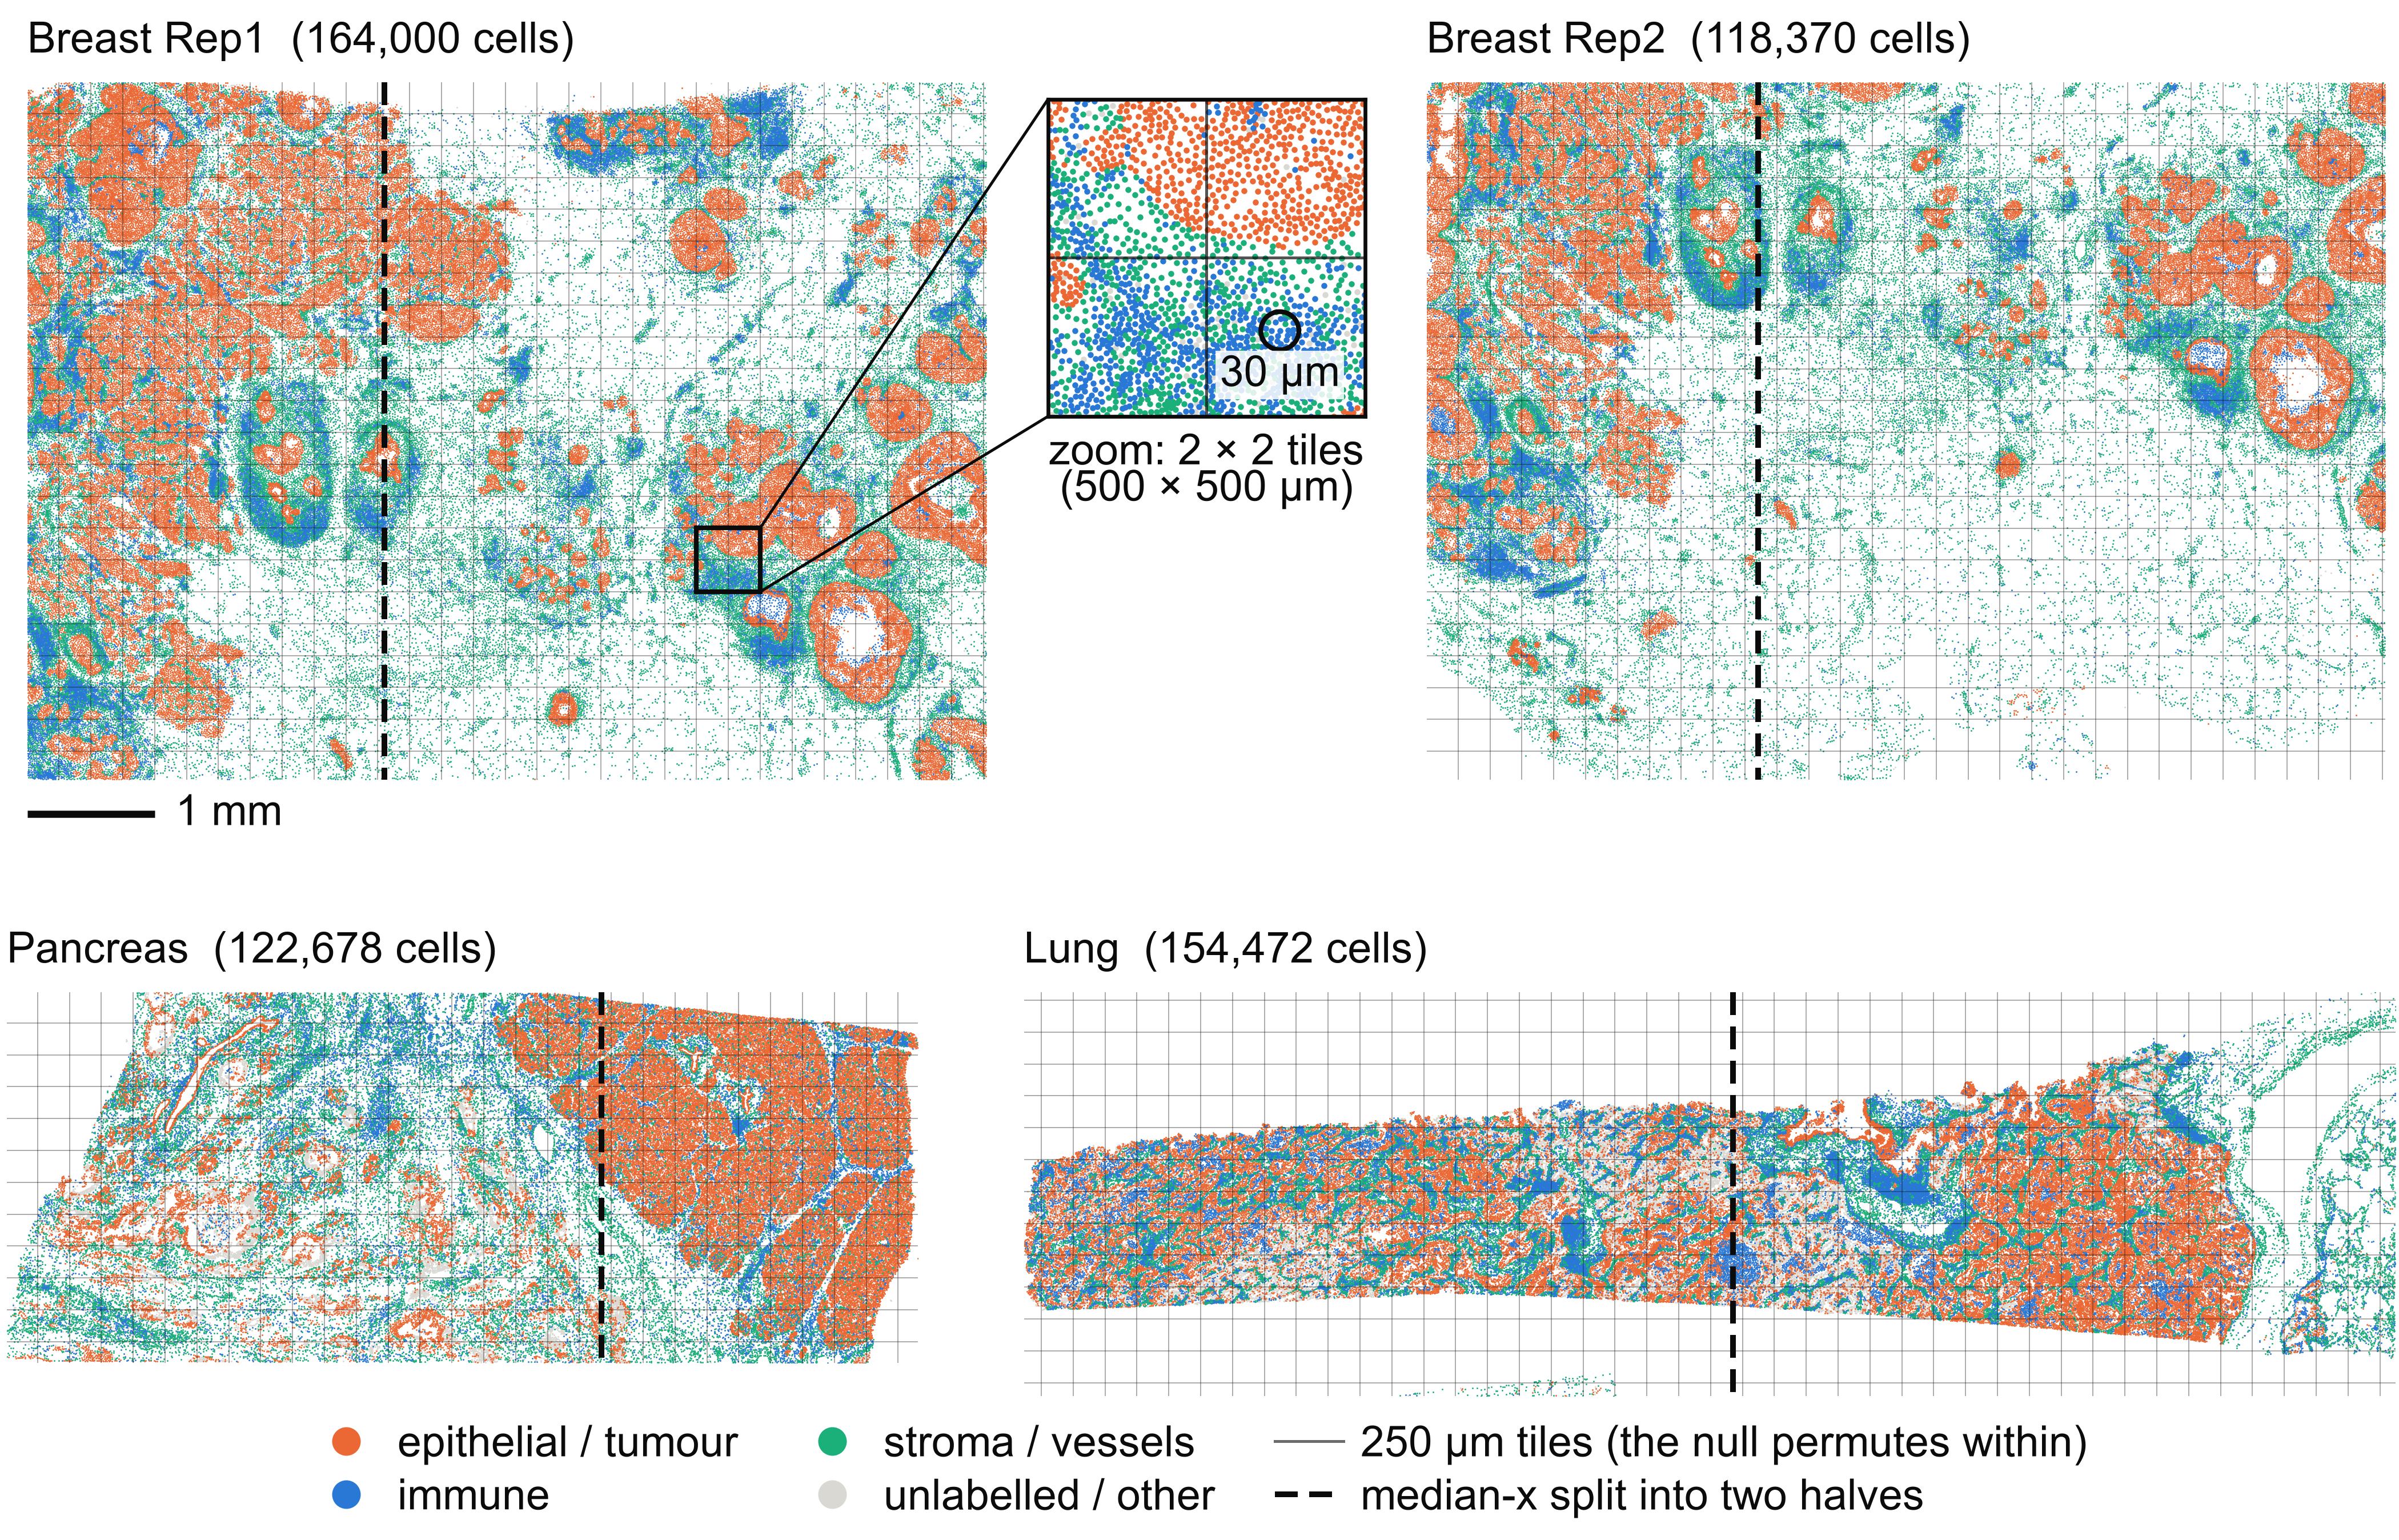
\includegraphics[width=\textwidth]{figures/figA4_tissues.png}
\caption{The four sections at one scale, coloured by broad compartment (for display only; the gate uses the fine cell
types). Grey lines: the gate's 250\um\ tiles, anchored at the origin. Dashed line: the median-$x$ split into two
halves. Inset: a $2\times2$-tile window of breast Rep1 with the 30\um\ interaction range drawn around one cell.}
\label{fig:tissues}
\end{figure*}

\begin{figure*}[t]
\centering
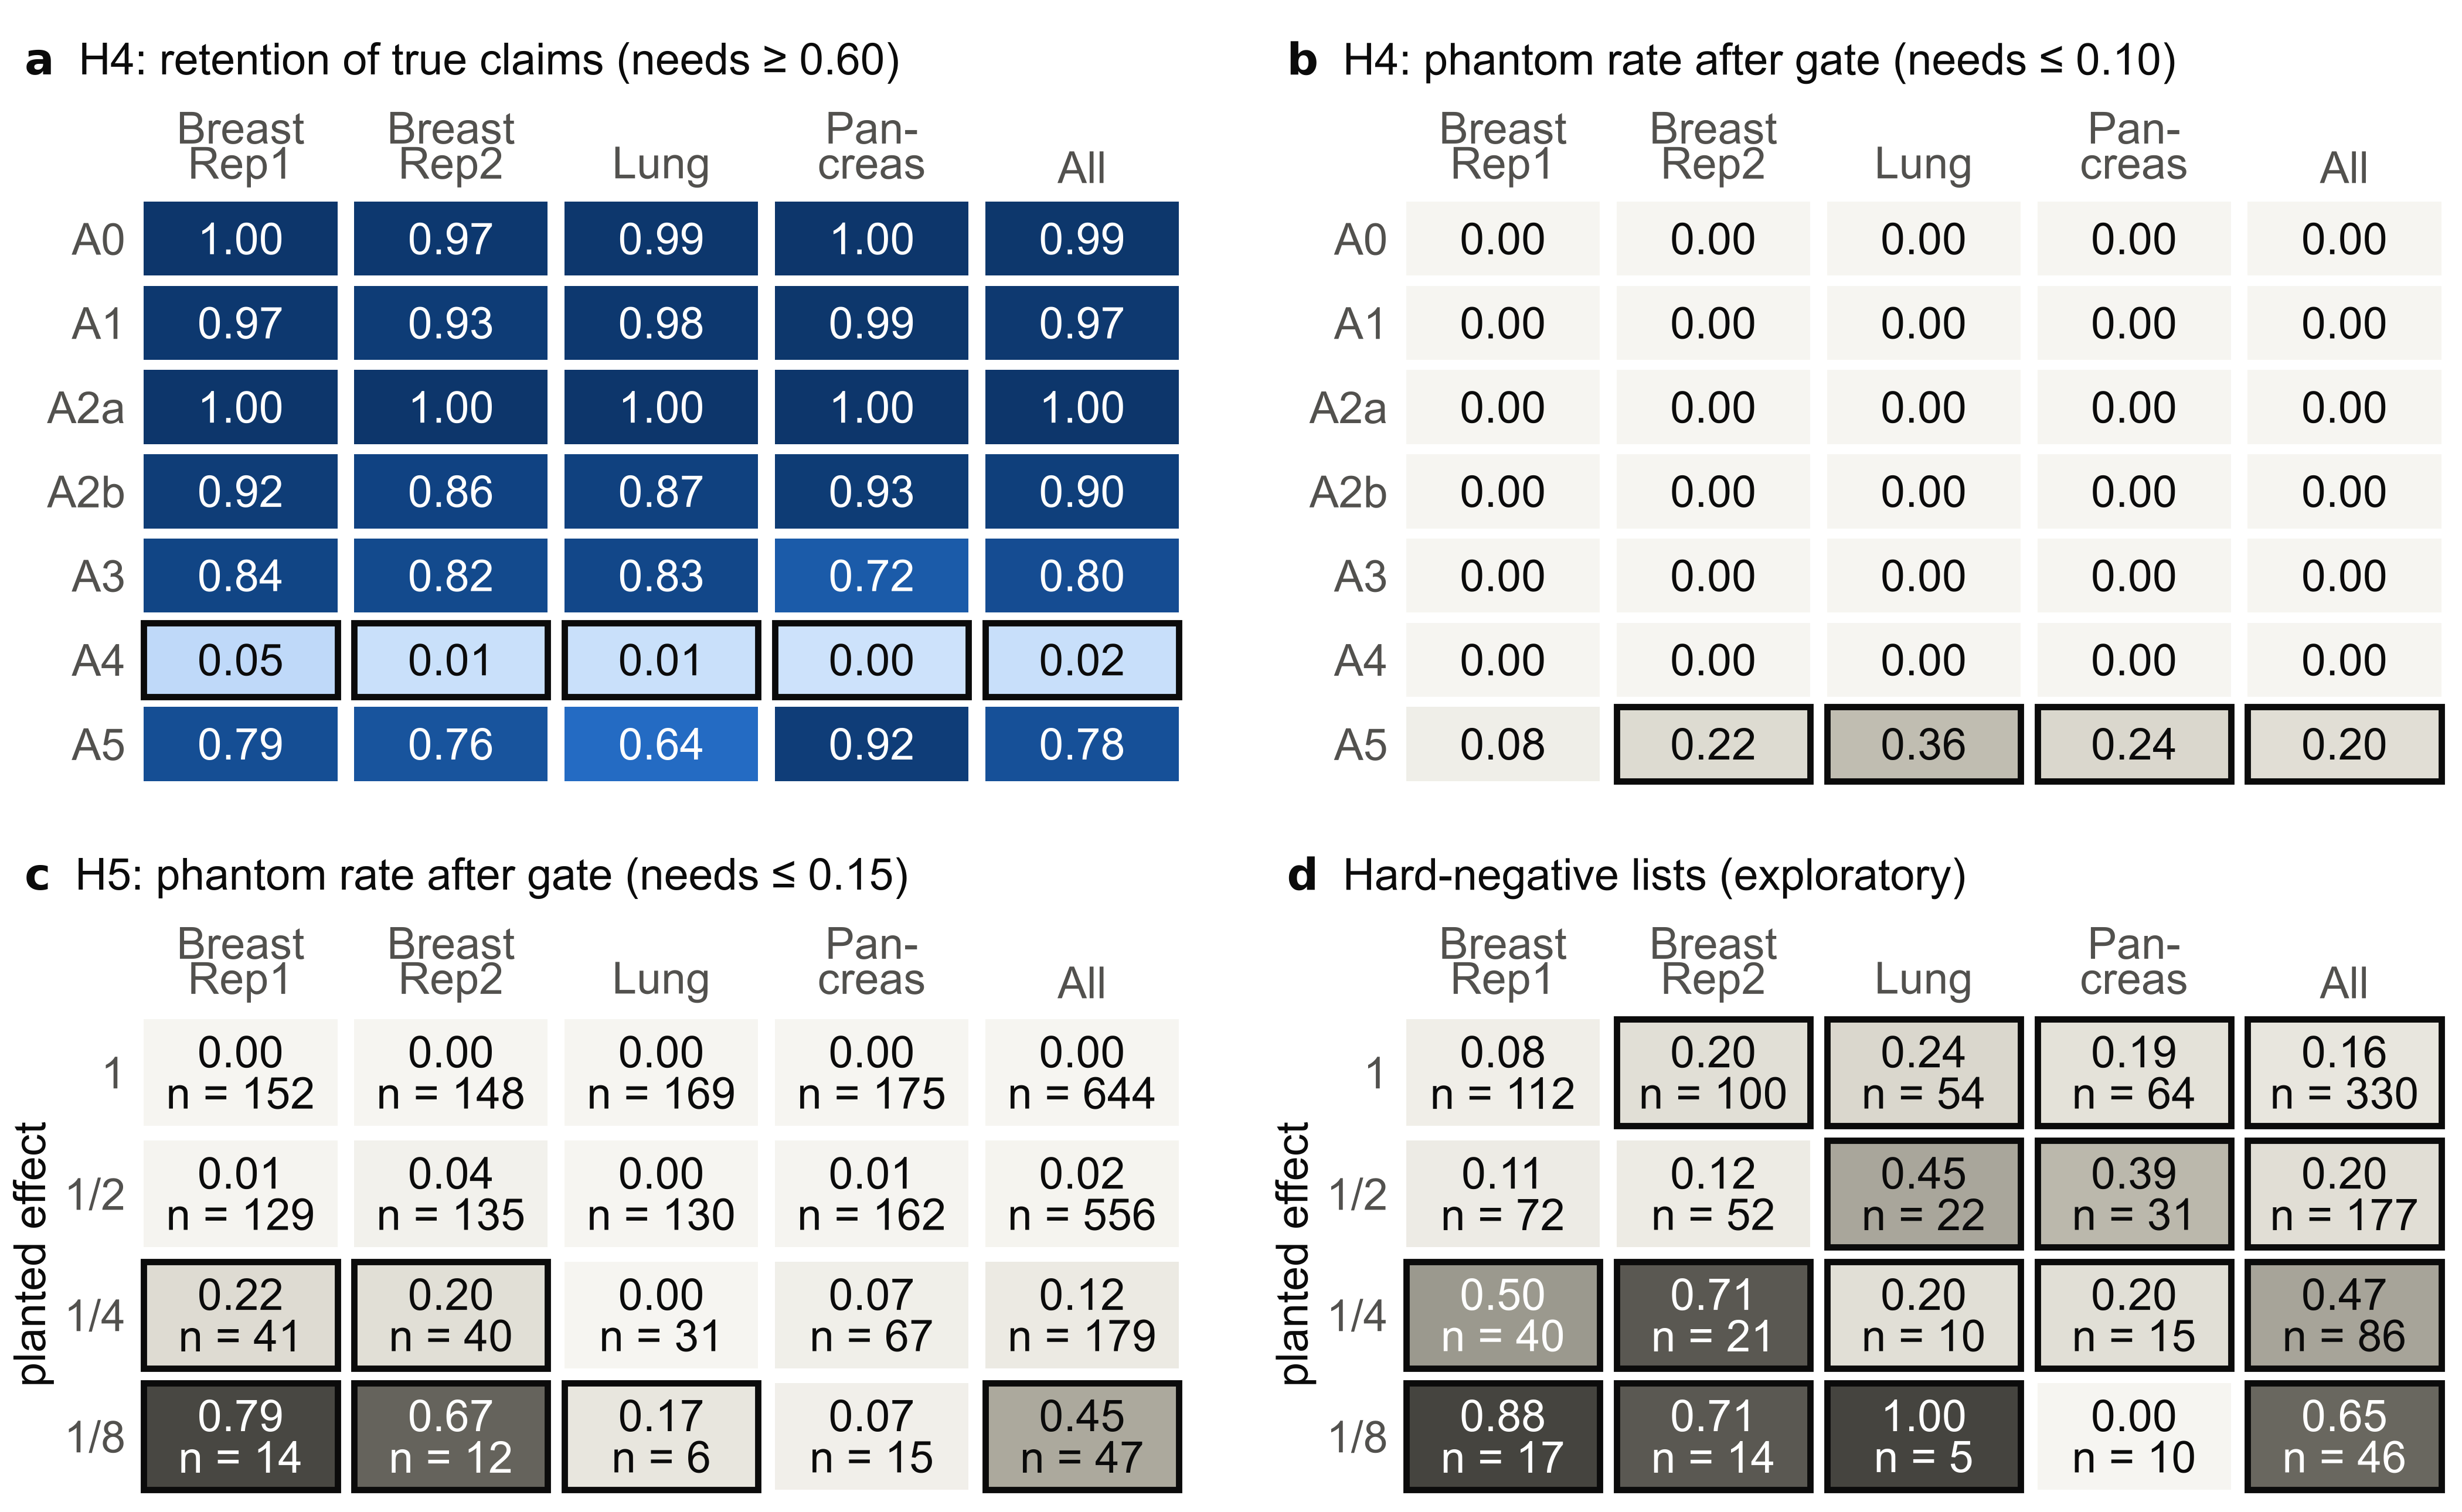
\includegraphics[width=\textwidth]{figures/figA6_per_tissue.png}
\caption{Per-tissue results on fresh seeds ($K{=}10$, cpdb and prod lists, seeds 200--209 pooled within each tissue).
Outlined cells miss the pre-registered threshold. (a, b) H4 retention and post-gate phantom rate for each variant.
(c) H5 post-gate phantom rate for each effect level, with the number of passed claims behind each rate. (d) The same
for the exploratory hard-negative lists; the outline uses the H5 threshold for reference only.}
\label{fig:pertissue}
\end{figure*}

\subsection{Library Size and Local Density}
Figure~\ref{fig:libsize} shows the association behind the normalisation account of the failure map. In breast Rep1,
cells with more neighbours carry fewer counts, and this holds within each broad compartment (Spearman $\rho$
\lcBreastReponeEpithelialTumourRho{} for epithelial and tumour cells, \lcBreastReponeImmuneRho{} for immune cells and
\lcBreastReponeStromaVesselsRho{} for stroma and vessels), so it is not only a matter of which cell types are dense.
Dividing by library size therefore inflates the normalised expression of crowded cells. In pancreas the positive
association is mostly one of composition: epithelial and tumour cells are the most crowded (median
\lcPancreasEpithelialTumourDens{} neighbours within 30\um) and carry larger libraries (\lcPancreasEpithelialTumourLib{}
times the section median), while within each compartment $\rho$ lies between \lcPancreasEpithelialTumourRho{} and
\lcPancreasImmuneRho{}. Either way, a response normalised by library size can follow crowding rather than signalling,
in a direction that depends on the tissue. The maps, curves and compartment values use all cells (record
\texttt{laneL\_libsize\_density\_by\_compartment}); the correlations printed in panel (b) are the logged values from
the Phase~2 diagnostic, computed on a cell sample.

\begin{figure*}[t]
\centering
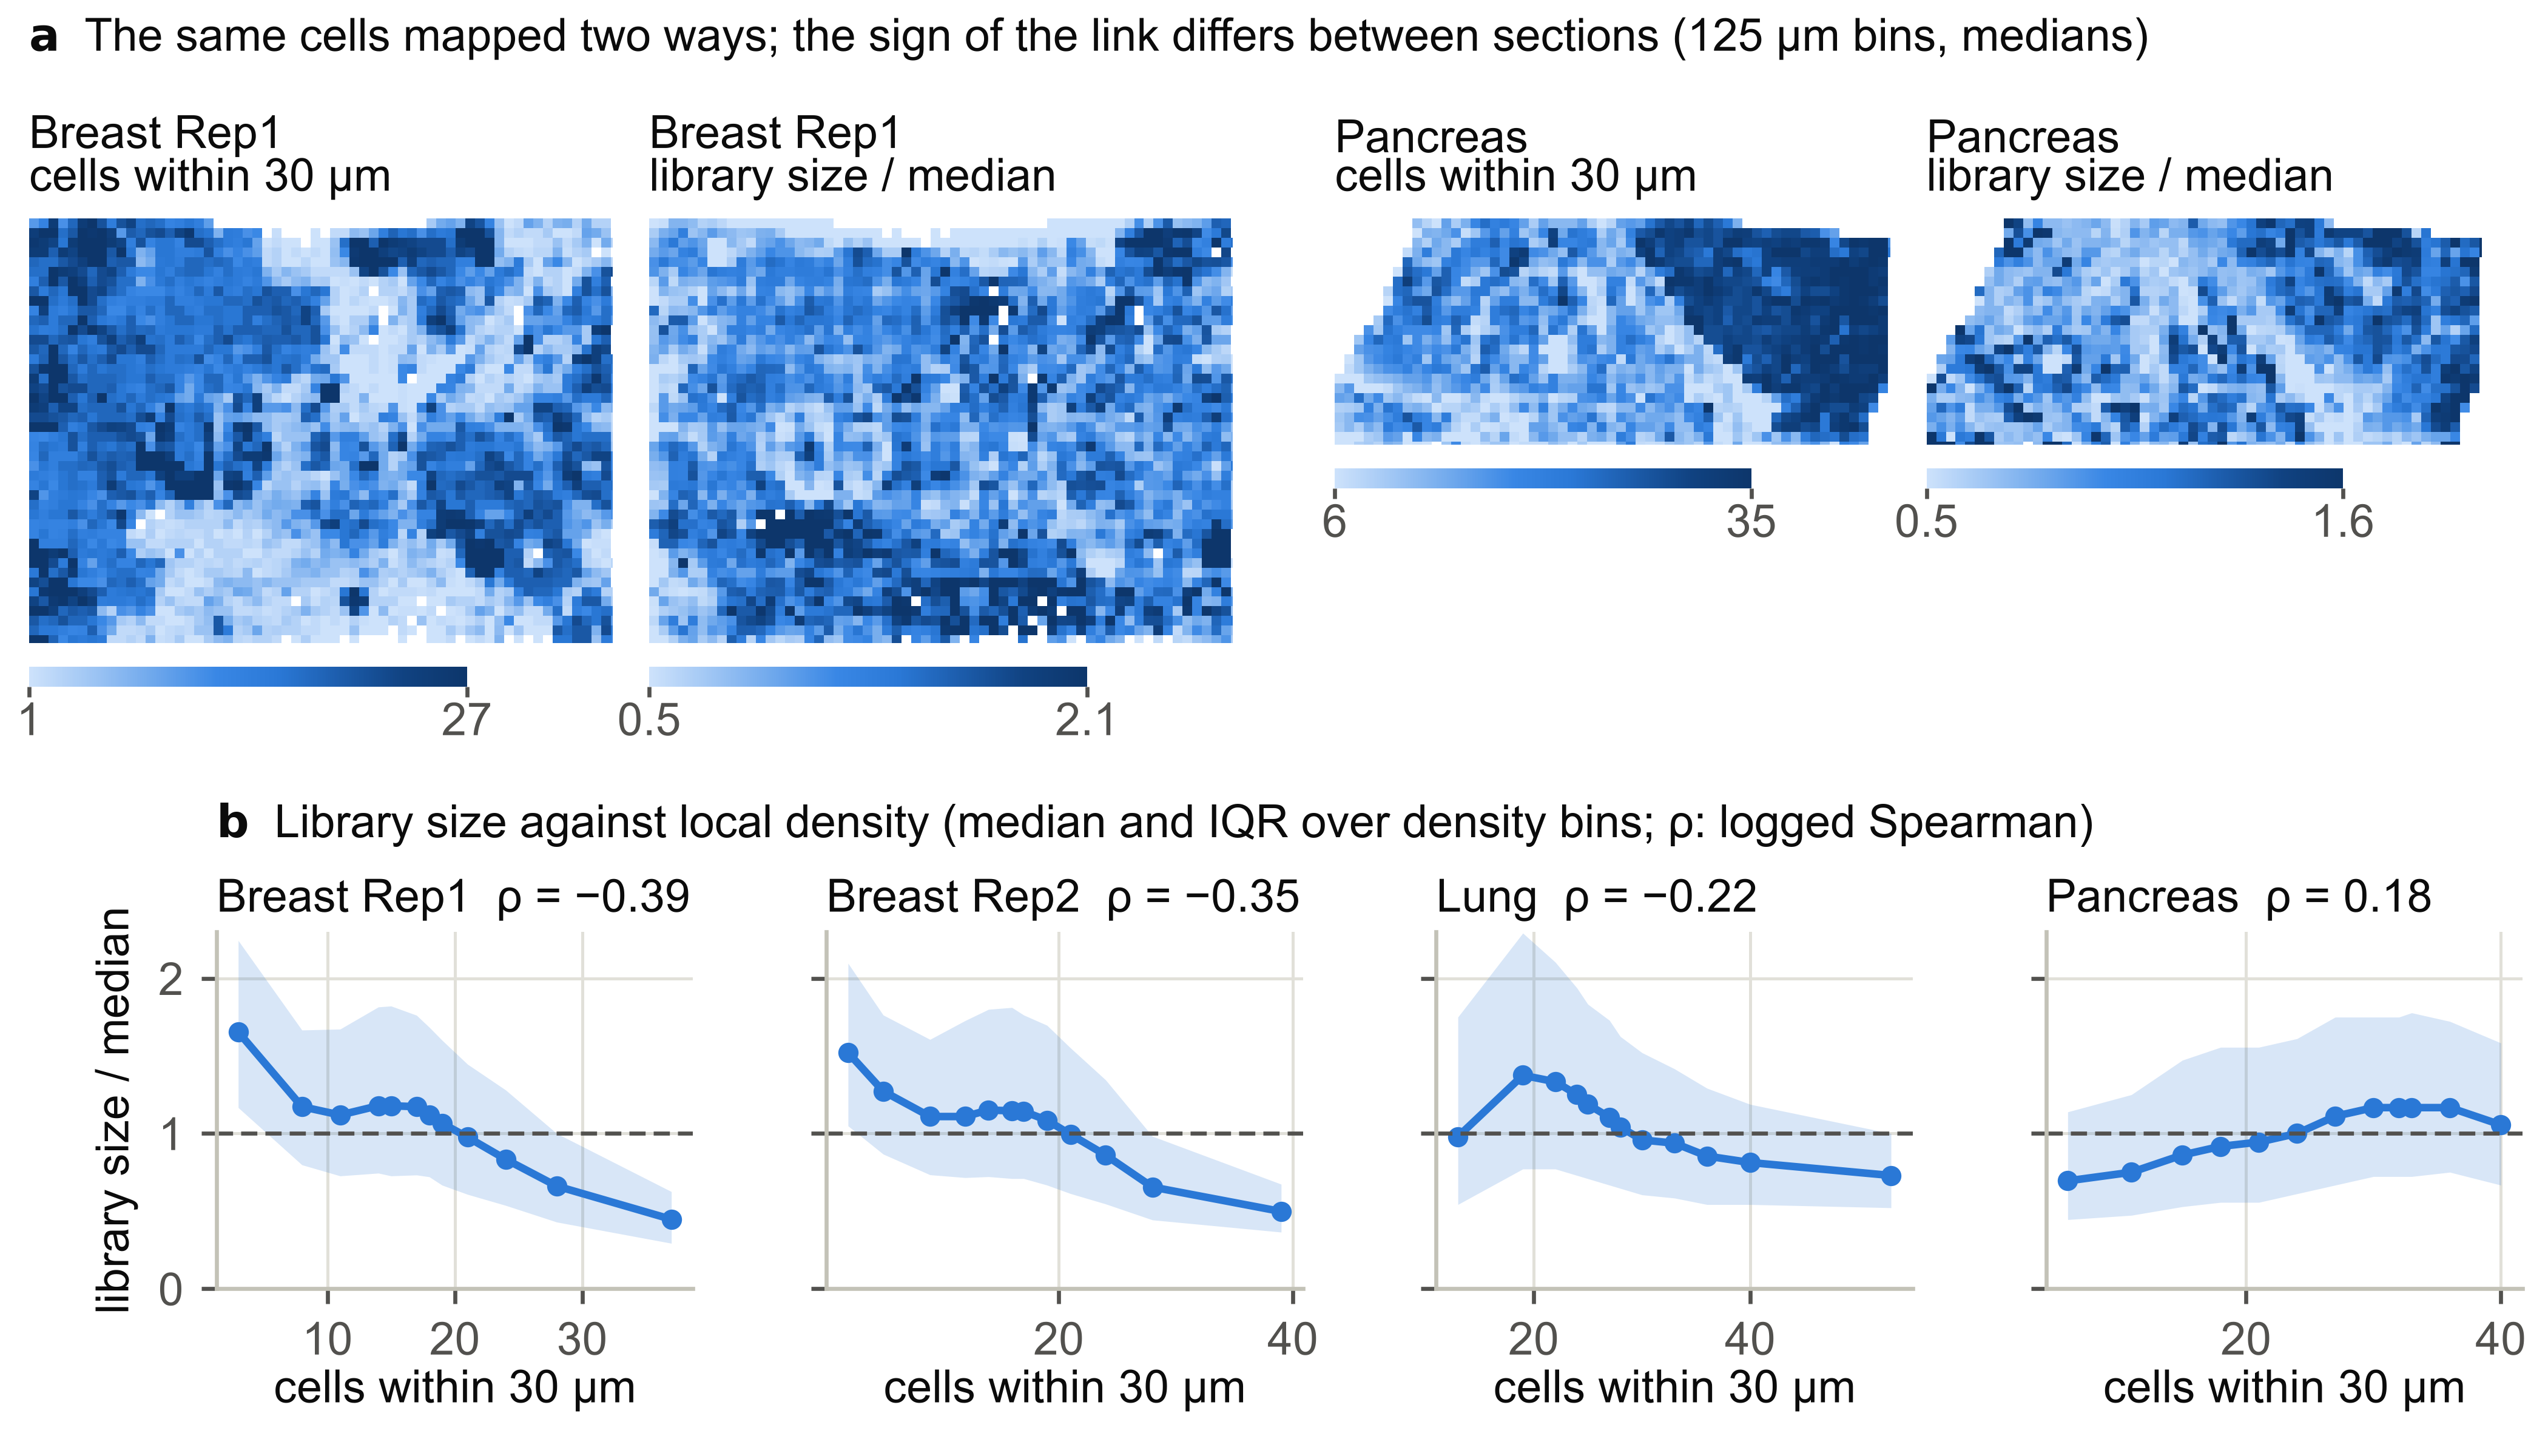
\includegraphics[width=\textwidth]{figures/figA5_libsize_density.png}
\caption{Library size and local density. (a) Median number of cells within 30\um\ and median library size relative to
the section median, in 125\um\ bins, for breast Rep1 and pancreas (colour scales clipped at the 5th and 95th
percentiles). (b) Median and interquartile range of relative library size across density bins, all cells; $\rho$ is
the logged Spearman correlation between library size and density.}
\label{fig:libsize}
\end{figure*}

\subsection{Sensitivity Analyses (Exploratory)}
Table~\ref{tab:sens} and Figure~\ref{fig:sens} change one setting of the frozen gate at a time on the dev seeds of
breast Rep1; nothing here was fed back into the gate. Results that change the picture: the tile size and range trade
retention against false passes (smaller tiles and shorter ranges lose true claims; larger tiles admit more hard
negatives); the minimum-evidence threshold never binds in these lists; a checkerboard split admits more hard
negatives than the left/right split; and a density-stratified null removes few of the hard-niche passes
(\senNullDensityNicheHard{} against \senFrozenNicheHard{} of \senNicheHardN{}) while lowering retention. Computing the
response from raw counts removed all hard-niche passes (\senRespRawNicheHard{}), which supports the normalisation
account but is partly matched to how the generator plants counts. \emph{Border tiles}: a tile is a border tile if one
of its eight neighbours holds no cell; for the median claim \edgeMedFrac{} of the receivers lie in border tiles.
Dropping those receivers changed \edgeNFlipped{} of \edgeNClaims{} decisions (\edgeNPassToFail{} passes became fails
and \edgeNFailToPass{} fails became passes).

\begin{table*}[t]
\centering
\small
\begin{tabular}{@{}lllll@{}}
\toprule
setting & A0--A3 retention & A5 retention & A5 phantom rate after gate & A5 hard-niche / decoy pass rate \\
\midrule
frozen gate & 0.94 [0.89, 0.98] & 0.67 [0.48, 0.88] & 0.23 [0.04, 0.44] & 0.18 / 0.00 \\
tiles 125\um & 0.81 [0.74, 0.87] & 0.67 [0.48, 0.88] & 0.20 [0.02, 0.38] & 0.16 / 0.00 \\
tiles 500\um & 0.95 [0.91, 0.98] & 0.73 [0.55, 0.93] & 0.31 [0.10, 0.52] & 0.24 / 0.12 \\
range 15\um & 0.78 [0.67, 0.87] & 0.53 [0.38, 0.69] & 0.24 [0.00, 0.45] & 0.12 / 0.00 \\
range 60\um & 0.93 [0.88, 0.97] & 0.73 [0.55, 0.93] & 0.22 [0.00, 0.43] & 0.20 / 0.08 \\
min.\ contacts 25 & 0.94 [0.89, 0.98] & 0.67 [0.48, 0.88] & 0.23 [0.04, 0.44] & 0.18 / 0.00 \\
min.\ contacts 100 & 0.94 [0.89, 0.98] & 0.67 [0.48, 0.88] & 0.23 [0.04, 0.44] & 0.18 / 0.00 \\
checkerboard halves & 0.92 [0.86, 0.97] & 0.69 [0.50, 0.91] & 0.29 [0.07, 0.52] & 0.28 / 0.08 \\
global null & 0.99 [0.98, 1.00] & 0.78 [0.62, 0.94] & 0.39 [0.22, 0.56] & 0.50 / 0.12 \\
density-stratified null & 0.82 [0.75, 0.89] & 0.67 [0.48, 0.88] & 0.20 [0.02, 0.40] & 0.14 / 0.00 \\
border tiles dropped & 0.91 [0.86, 0.96] & 0.69 [0.50, 0.91] & 0.26 [0.04, 0.47] & 0.22 / 0.04 \\
raw-count response & 0.88 [0.81, 0.94] & 0.67 [0.48, 0.88] & 0.00 [0.00, 0.00] & 0.00 / 0.00 \\
\bottomrule
\end{tabular}
\caption{Sensitivity of the frozen gate's decisions (exploratory; dev seeds 0, 1, 2, 3, 4 of breast Rep1; one setting changed at a time; $K{=}10$ lists of both expression tools; 95\% hierarchical bootstrap CIs). Hard-niche and decoy pass rates are over all planted A5 claims of that kind. Source: results record \texttt{laneR\_dev\_sensitivity}.}
\label{tab:sens}
\end{table*}


\begin{figure*}[t]
\centering
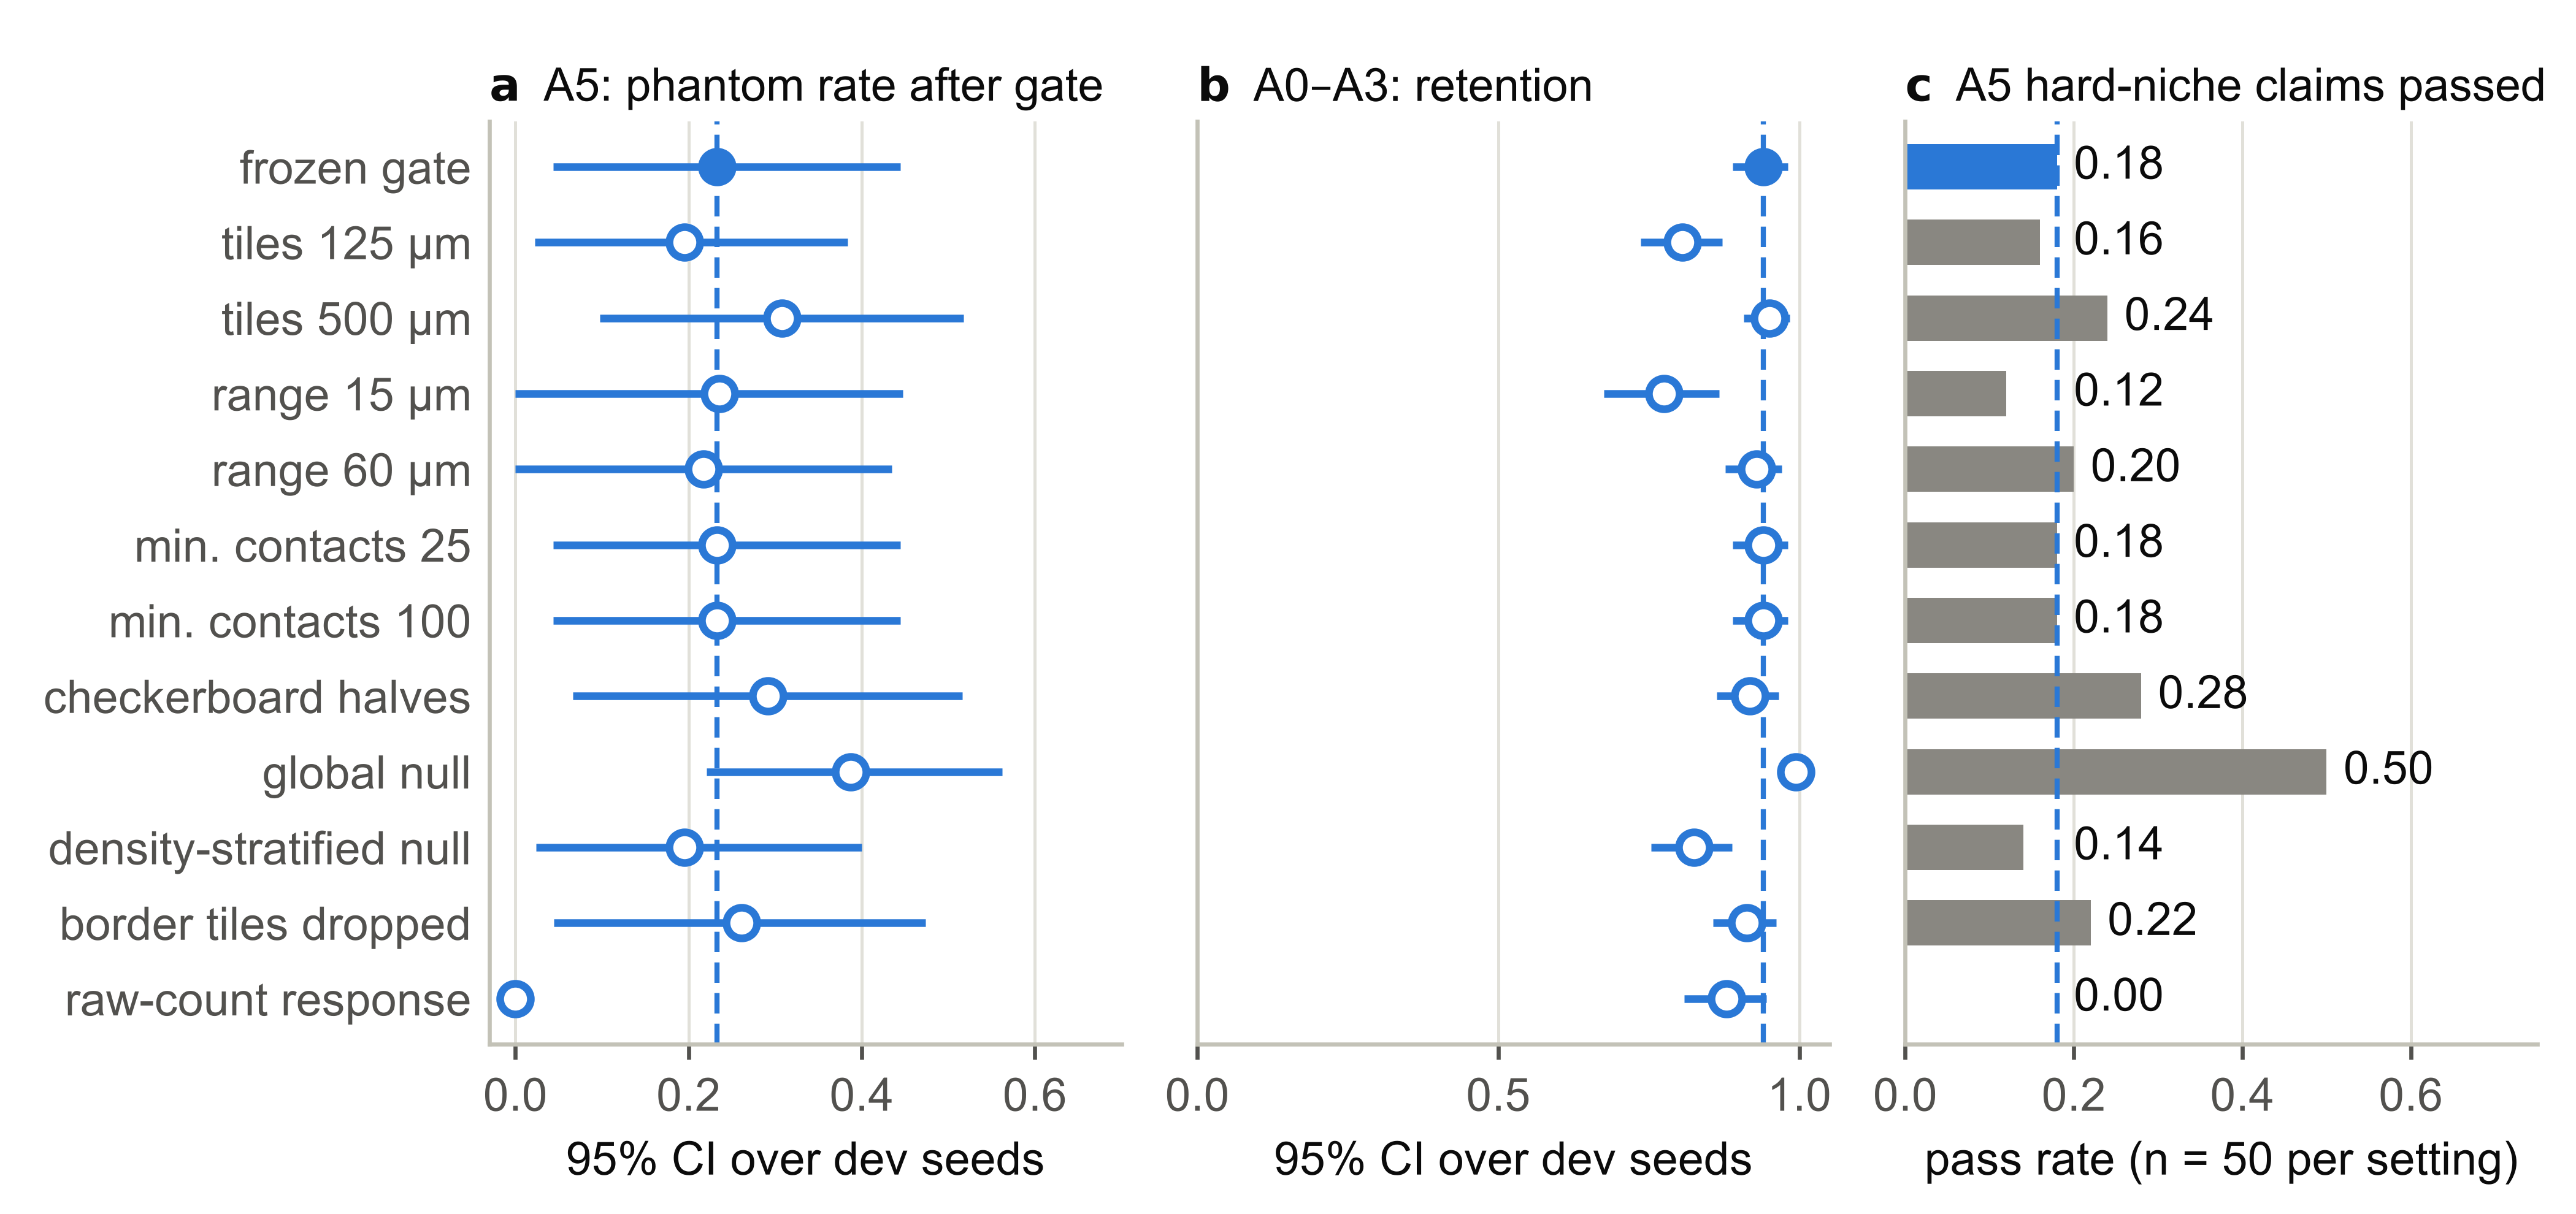
\includegraphics[width=\textwidth]{figures/figA3_sensitivity.png}
\caption{Sensitivity of the frozen gate (exploratory; dev seeds 0--4, breast Rep1; one setting changed at a time).
(a) Post-gate phantom rate on A5 lists and (b) retention on A0--A3 lists, with 95\% CIs; the dashed line marks the
frozen gate. (c) Pass rate of the planted A5 hard-niche claims.}
\label{fig:sens}
\end{figure*}

\subsection{Pre-registration Record and the Amendment~4 Timestamp}
Amendments 1--3 (Phase~1) restricted the donor-gene range after a degenerate first smoke run, froze the tuned gate
configuration (equal to the defaults), and documented behaviour-preserving code edits after the freeze. Amendment~4
registered H4--H7 and the N2 seeds. Its header gives the time ``2026-11-07 15:00 CST'', which was not read from a clock.
The amendment was first committed at 2026-11-07 23:57:32 CST (commit \texttt{216b498}); the commit time is
authoritative. The order that pre-registration requires still holds: the H4 analysis specification was committed at
2026-11-08 00:08:52, and the first N2 benchmark instance was written at 00:12:11. We left the amendment text unchanged
and appended an erratum to the pre-registration document. The H5 specification was committed before any N2 instance
with an effect below 1 existed; the full-effect N2 lists had already been seen through H4's reference variant, which we
disclosed in that specification.

\subsection{Phase 1 Details}
Table~\ref{tab:verdicts} gives the Phase~1 verdict for every condition and split, and Figure~\ref{fig:phase1} shows the
phantom rates and the gate's pass rates on all planted claims. On dev, removing the tile restriction raised the niche
pass rate from \plantedFullNiche{} to \plantedNoTilesNiche{}. On hard dev lists of all ten true and all ten niche
claims (exploratory), the frozen gate gave a post-gate phantom rate of \hardFullPRafter{}, against \hardNoTilesPRafter{}
without tile restriction. With the receptor as the only readout (the situation on real data), retention on the
benchmark fell to \swDefaultReceptorOnlyCpdbRet{} \swDefaultReceptorOnlyCpdbRetci{}, and with no responding target to
\swRespzeroNoneCpdbRet{}.

\begin{table*}[t]\centering\small
\begin{tabular}{llllllll}\toprule
split & tissue & condition & phantom@10 & H1 & after gate & retention & H2\\\midrule
dev & breast\_rep1 & expr\_cpdb & 0.30 [0.16, 0.46] & INCONCLUSIVE & 0.00 & 0.97 [0.88, 1.00] & SUPPORTED\\
dev & breast\_rep1 & expr\_prod & 0.24 [0.12, 0.38] & INCONCLUSIVE & 0.00 & 0.97 [0.88, 1.00] & SUPPORTED\\
dev & breast\_rep1 & agent\_gemini & 0.27 [0.07, 0.53] & INCONCLUSIVE & 0.00 & 0.95 [0.81, 1.00] & SUPPORTED\\
dev & breast\_rep1 & agent\_deepseek & 0.13 [0.03, 0.27] & INCONCLUSIVE & 0.00 & 0.96 [0.84, 1.00] & SUPPORTED\\
dev & breast\_rep1 & agent\_both & 0.20 [0.07, 0.35] & INCONCLUSIVE & 0.00 & 0.96 [0.87, 1.00] & SUPPORTED\\
test & breast\_rep1 & expr\_cpdb & 0.20 [0.08, 0.32] & INCONCLUSIVE & 0.00 & 1.00 [1.00, 1.00] & SUPPORTED\\
test & breast\_rep1 & expr\_prod & 0.20 [0.08, 0.34] & INCONCLUSIVE & 0.00 & 1.00 [1.00, 1.00] & SUPPORTED\\
test & breast\_rep2 & expr\_cpdb & 0.18 [0.06, 0.32] & INCONCLUSIVE & 0.00 & 1.00 [1.00, 1.00] & SUPPORTED\\
test & breast\_rep2 & expr\_prod & 0.18 [0.06, 0.32] & INCONCLUSIVE & 0.00 & 1.00 [1.00, 1.00] & SUPPORTED\\
test & pancreas & expr\_cpdb & 0.12 [0.04, 0.22] & INCONCLUSIVE & 0.00 & 1.00 [1.00, 1.00] & SUPPORTED\\
test & pancreas & expr\_prod & 0.12 [0.04, 0.22] & INCONCLUSIVE & 0.00 & 1.00 [1.00, 1.00] & SUPPORTED\\
\bottomrule\end{tabular}
\caption{Pre-registered verdicts (K=10; 95\% hierarchical bootstrap CIs). H3: NOT YET RUN.}\label{tab:verdicts}
\end{table*}


\begin{figure*}[t]
\centering
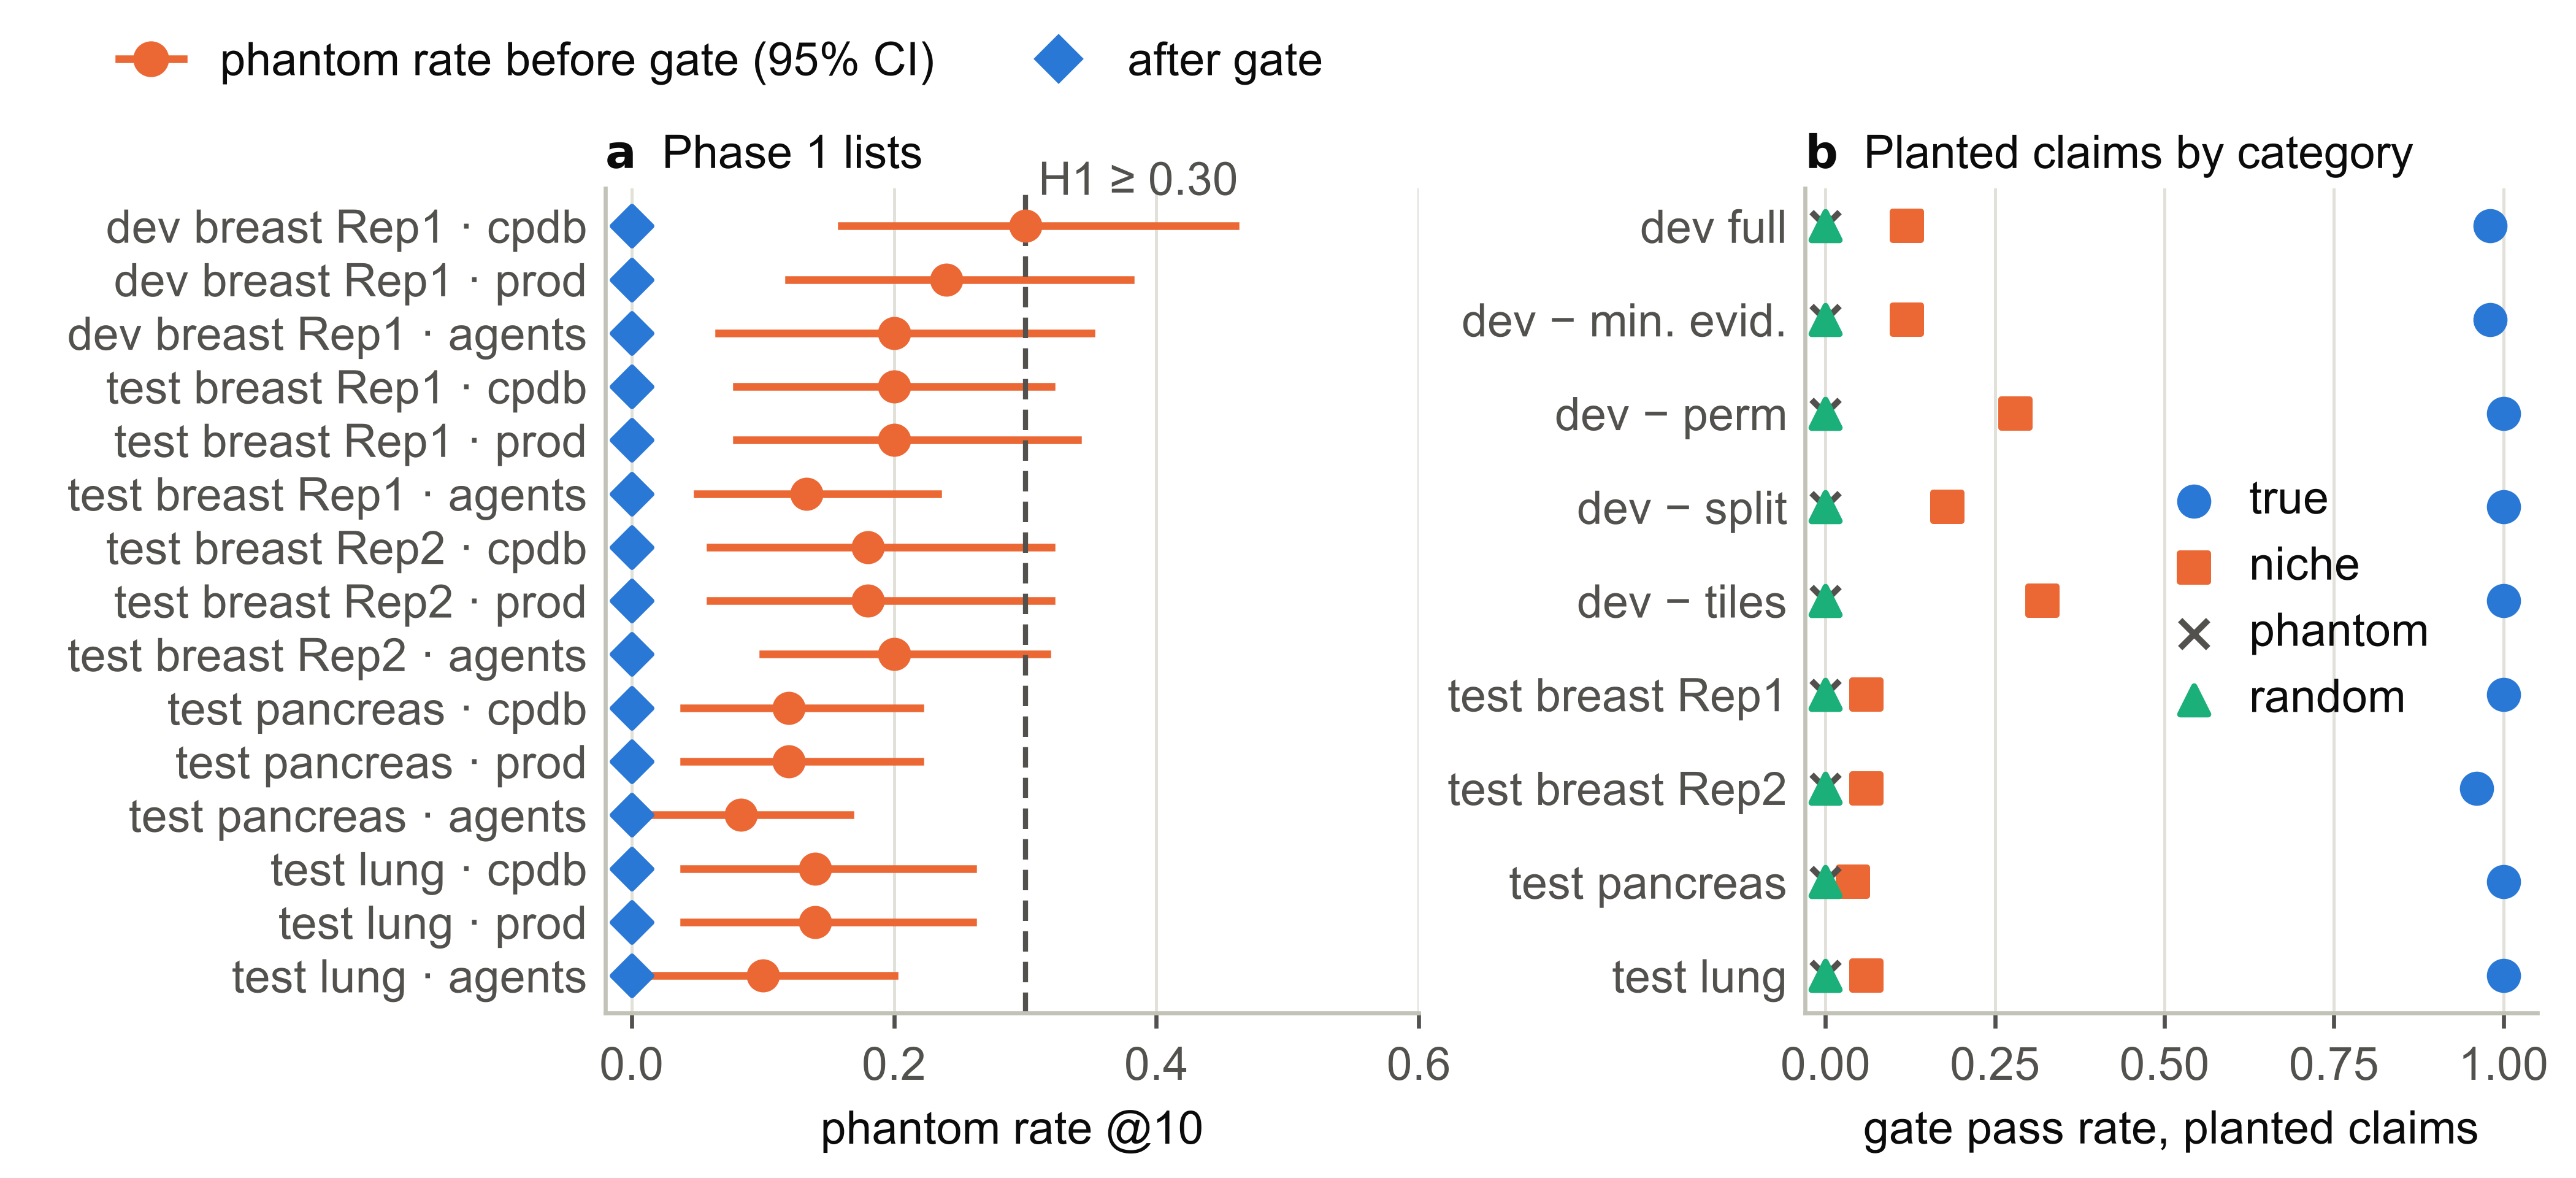
\includegraphics[width=\textwidth]{figures/figA1_phase1.png}
\caption{Phase~1. (a) Phantom rate at $K{=}10$ before (95\% CI) and after the frozen gate for each split and condition
(agents: both families pooled). (b) Gate pass rate on all planted claims by category: dev ablations and held-out test
tissues.}
\label{fig:phase1}
\end{figure*}

\begin{figure}[t]
\centering
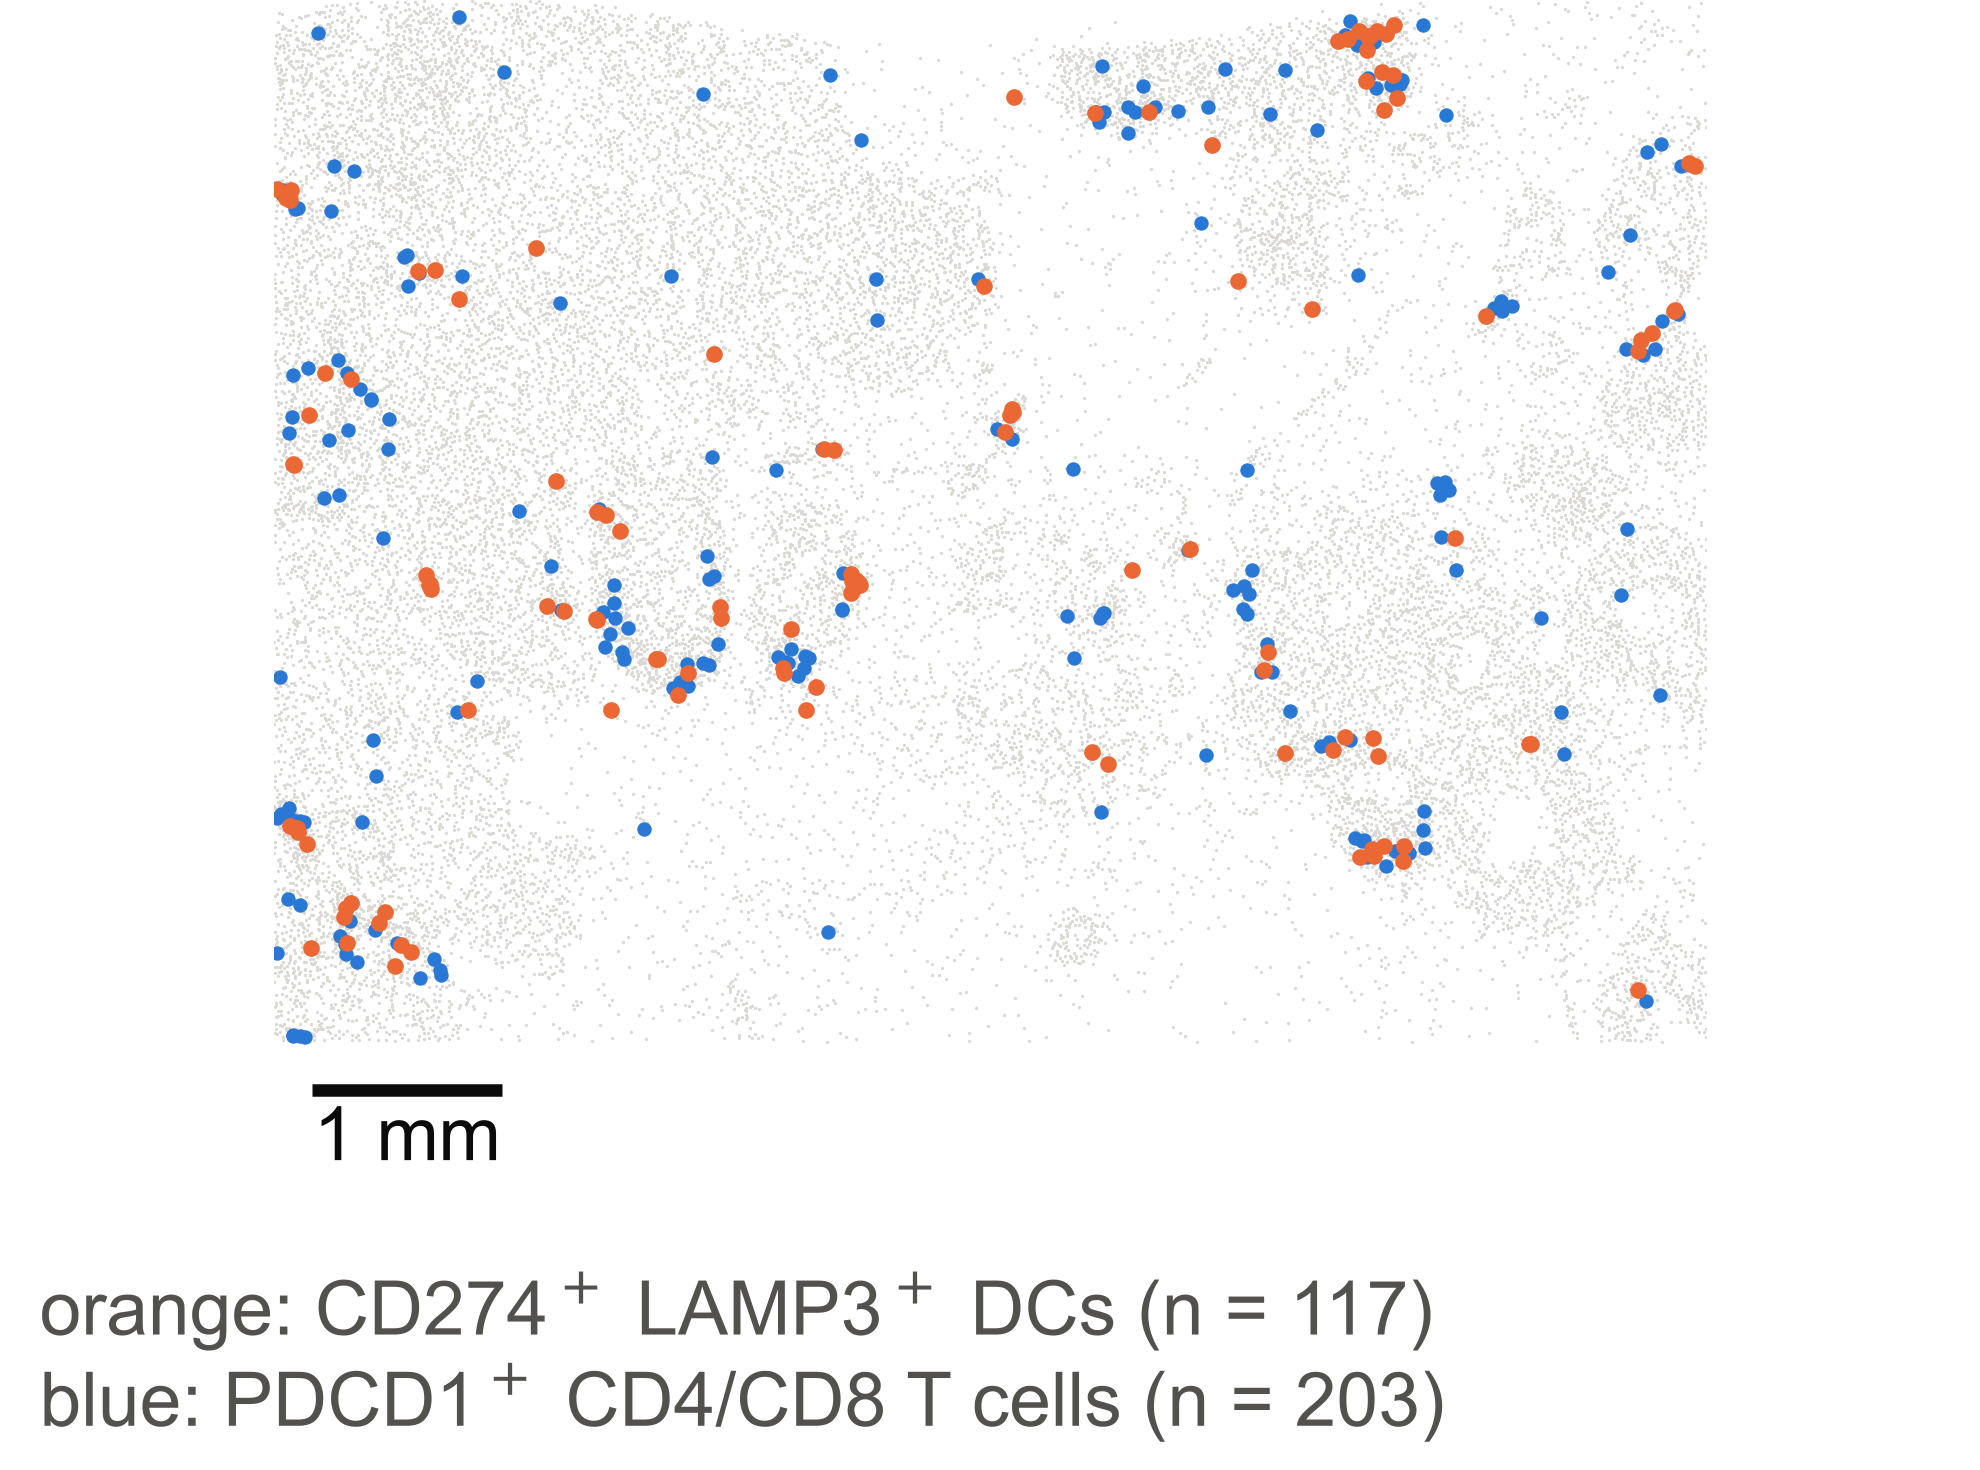
\includegraphics[width=\columnwidth]{figures/figA2_real_pdl1.png}
\caption{Real breast Rep1, no planting: CD274$^+$ (PD-L1) LAMP3$^+$ dendritic cells and PDCD1$^+$ (PD-1) T cells,
the type pairs an expression tool ranks highest for PD-L1/PD-1. Their contacts are few, and at chance level
(observed/expected \realContactRatioLo{}--\realContactRatioHi{}).}
\label{fig:pdl1}
\end{figure}

\subsection{Example Audit Records}
Two records from the held-out breast evaluation (\texttt{results/audit/test\_final\_breast\_rep1\_cpdb\_K10\_none.jsonl})
and one from the real-data check (\texttt{results/audit/real\_breast\_gate.jsonl}); fields abridged, numbers rounded.
The last three fields come from the output-only status module (\texttt{gate/status.py}), which reads the frozen gate's
fields after the decision; rerunning every H4 cell with it gave identical decisions (Appendix, Reproducibility). A
planted true claim:
{\scriptsize\begin{verbatim}
{"claim": {"sender": "Macrophages_1", "receiver": "CD4+_T_Cells", "ligand": "LIG_38",
 "receptor": "REC_38"}, "response": {"targets": ["TGT_38_a", "TGT_38_b", "TGT_38_c"]},
 "n_expressing_pairs_within_r": 13147, "rho_within_tile": 0.3684, "p_perm": 0.001,
 "q_bh": 0.0011, "halves": [{"rho": 0.3716, "p": 0.001}, {"rho": 0.3657, "p": 0.001}],
 "pass_": true, "reasons": [], "status": "pass", "readout": "targets",
 "status_note": "state supports the claim through the measured readout"}
\end{verbatim}}
\noindent A planted phantom reported by an expression-only tool:
{\scriptsize\begin{verbatim}
{"claim": {"sender": "Myoepi_KRT15+", "receiver": "LAMP3+_DCs", "ligand": "LIG_36",
 "receptor": "REC_36"}, "response": {"targets": ["TGT_36_a", "TGT_36_b", "TGT_36_c"]},
 "n_expressing_pairs_within_r": 0, "rho_within_tile": 0.0, "p_perm": 1.0, "q_bh": 1.0,
 "pass_": false, "reasons": ["perm_null_not_rejected(q=1>0.05)", "split_inconsistent",
 "too_few_expressing_pairs(0<50)", "effect_below_min(rho=0<0.02)"], "status": "fail",
 "readout": "targets", "status_note": "measured readout does not support the claim"}
\end{verbatim}}
\noindent A real PD-L1/PD-1 claim on breast Rep1 (no target of the pair is on the panel, so the gate falls back to the
receptor's own expression):
{\scriptsize\begin{verbatim}
{"claim": {"sender": "LAMP3+_DCs", "receiver": "CD8+_T_Cells", "ligand": "CD274",
 "receptor": "PDCD1"}, "response": {"receptor": "PDCD1"}, "n_expressing_pairs_within_r": 11,
 "rho_within_tile": 0.0157, "p_perm": 0.118, "q_bh": 0.589, "pass_": false,
 "reasons": ["perm_null_not_rejected(q=0.589>0.05)", "split_inconsistent",
 "too_few_expressing_pairs(11<50)", "effect_below_min(rho=0.0157<0.02)"],
 "status": "untestable", "readout": "receptor_only",
 "status_note": "no downstream readout measured: no evidence either way"}
\end{verbatim}}

\subsection{Agent Protocol}
System prompt (abridged): ``You are a computational biology agent analysing a spatial transcriptomics section
(10x Xenium, single-cell resolution, coordinates in micrometres) \ldots{} gene names are anonymized \ldots{} each pair
lists putative downstream target genes \ldots{} at most 24 tool calls in total. Finish by calling submit\_claims
exactly once.'' Task: ``Report the top-10 cell-cell interactions in this tissue with evidence \ldots{} Call
submit\_claims with exactly 10 claims ranked from most to least confident.'' Tools: \texttt{list\_cell\_types},
\texttt{list\_lr\_database}, \texttt{expression\_summary}, \texttt{top\_expressed\_pairs} (CellPhoneDB-like ranking),
\texttt{spatial\_proximity}, \texttt{colocalization}, \texttt{compare\_near\_far} and \texttt{submit\_claims}, plus
\texttt{verify\_claim} in the gate-as-tool condition. Temperature 0.2, at most 12 turns. Full transcripts, including
every tool call and result, are in \texttt{results/agent\_logs/}. API keys were read from the environment at run time and
never logged.

\subsection{Cell-Type Annotation of Pancreas and Lung}
No published labels exist for these sections. Each vendor graph-based cluster was assigned the lineage whose marker set
had the highest mean $z$-scored log expression (for example T cells: CD3D, CD3E, CD2, TRAC; macrophages: CD68, CD163,
MRC1, MARCO; endothelial: PECAM1, VWF, CLEC14A; epithelial and tumour: EPCAM, KRT7, KRT20, CFTR; plus acinar and
endocrine markers for pancreas and ciliated and alveolar markers for lung). A cluster was left unlabelled if its best
score was below 0.3 or less than 0.1 above the runner-up; this rule was fixed before any evaluation.

\end{document}
